\chapter{Análise Exploratória}
\label{cap:analise_exploratoria}

Na primeira seção deste capítulo serão discutidos os resultados da análise de distribuição dos dados coletados, definindo para a API Android valores de referência em cada métrica. Na seção seguinte, é feito um trabalho de comparação de aplicativos com a API em função dos valores de referência definidos para a API em cada métrica. A primeira seção juntamente com a proposta de cálculo de similaridade da segunda seção reúnem as principais contribuições deste trabalho.

Na terceira seção, são apresentadas discussões sobre a possibilidade de validação dos valores de referência definidos no início deste capítulo através de regressão polinomial.

\section{Análise de Distribuição}

 \begin{figure}
        \centering
        \begin{subfigure}[b]{0.475\textwidth}
            \centering
            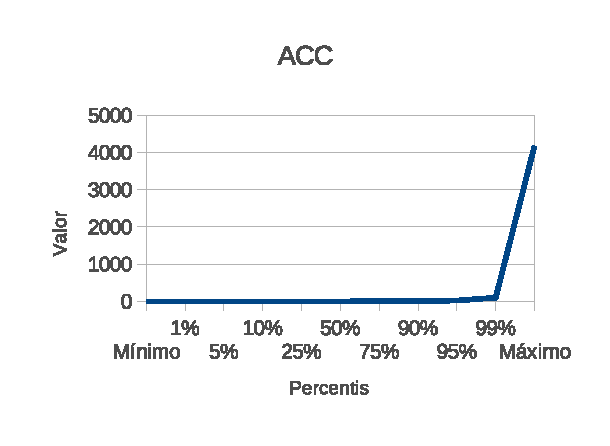
\includegraphics[width=\textwidth]{figuras/dist/acc.eps} 
        \end{subfigure}
        \hfill
        \begin{subfigure}[b]{0.475\textwidth}  
            \centering 
            \includegraphics[width=\textwidth]{figuras/dist/accm.eps}
        \end{subfigure}
        \vskip\baselineskip
        \begin{subfigure}[b]{0.475\textwidth}   
            \centering 
            \includegraphics[width=\textwidth]{figuras/dist/lcom4.eps}
        \end{subfigure}
        \quad
        \begin{subfigure}[b]{0.475\textwidth}   
            \centering 
            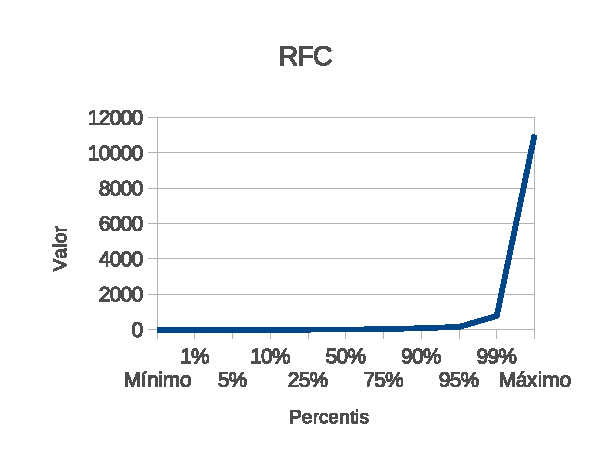
\includegraphics[width=\textwidth]{figuras/dist/rfc.eps}
        \end{subfigure}
        \caption[]
        {\small Distribuição das métricas ACC, ACCM, LCOM4 e RFC na versão 5.1.0} 
 \label{fig:android510dist}
    \end{figure}


Com os dados coletados e devidamente preparados, várias conclusões podem ser tiradas dos valores das métricas e sua evolução ao longo do tempo. Esta seção é focada na análise subjetiva dos dados, tentando explicar seu comportamento com relação às características do sistema, compará-los a outros estudos, e até mesmo comparar com dados de métricas em aplicativos, utilizando os próprios aplicativos do sistema como base de comparação.

\subsection{Distribuição dos dados}

Os gráficos na Figura~\ref{fig:android510dist} apresentam as distribuições dos dados para as métricas LCOM4, ACC, ACCM e RFC. Podemos perceber que em todos os casos a probabilidade cumulativa, representada pelos percentis, apresenta um aumento de valor apenas nos últimos percentis, já demonstrando que que esses valores nos últimos percentis são bem discrepantes. Entretanto eles só começam a realmente aumentar significativamente a partir do percentil 95, então os 5\% restantes podem ser descartados como um ruído estatístico. 

Nas tabelas que serão discutidas nas seção seguintes, percebe-se que a mediana, no percentil 50, não representa de forma alguma os dados como faria numa distribuição normal. Para muitas métricas esse percentil apresenta nada mais que o ideal teórico que na prática não é comum, como nas métricas ACCM, NOC, LCOM4 e ACC. Assim, serão utilizados percentis 75, 90 e 95 para análise cada métrica, assim como feito por \citeonline{meirelles2013}.

Valores considerados como 0 para muitas métricas não tem valor semântico para interpretação e resulta da impossibilidade de calcular a métrica. Resultado 0 para LCOM4, ACCM e RFC, por exemplo, indicam classes sem métodos.

\subsection{Average Method Lines Of Code}

\begin{table}[!htb]
\centering
\scalefont{.7}
\begin{tabular}{|l|l|l|l|l|l|l|l|l|l|l|l|l|}
\hline
versão&classes&min&1\%&5\%&10\%&25\%&50\%&75\%&90\%&95\%&99\%&max\\
\hline
android-1.6\_r1.2&5745&0&0&0&0&2.33&5.57&11.5&21.5&30&65.87&312\\
\hline
android-1.6\_r1.5&5745&0&0&0&0&2.33&5.57&11.5&21.5&30&65.87&312\\
\hline
android-2.0\_r1&6331&0&0&0&0&2&5.56&11.5&21.85&30.19&67.81&390.5\\
\hline
android-2.1\_r2.1p2&6360&0&0&0&0&2&5.63&11.5&21.86&30.34&68.4&395\\
\hline
android-2.2\_r1&7352&0&0&0&0&1.76&5.8&12.8&26.5&44.21&156.66&1034\\
\hline
android-2.2.3\_r2&7358&0&0&0&0&1.77&5.82&12.82&26.5&44.17&156.62&1034\\
\hline
android-2.3\_r1&8093&0&0&0&0&1&5.8&13.6&30.18&55.36&164.77&1034\\
\hline
android-2.3.7\_r1&8240&0&0&0&0&1&5.83&13.71&30&54.06&163.4&1034\\
\hline
android-4.0.1\_r1&11709&0&0&0&0&1&5.86&14&31&54.37&162.42&1034\\
\hline
android-4.0.4\_r2.1&11851&0&0&0&0&1&5.86&14&31&53.98&162&1034\\
\hline
android-4.1.1\_r1&14115&0&0&0&0&1&5.5&13.08&28.96&51&151.95&1034\\
\hline
android-4.3.1\_r1&15472&0&0&0&0&1&5.5&12.5&26.2&43&126&721\\
\hline
android-5.1.0\_r1&20129&0&0&0&0&2&5.5&12&24&37.8&105&708\\
\hline
\end{tabular}

\caption{\textit{Average Method Lines of Code} no Android}
\label{tab:amloc_android}
\end{table}

\begin{figure}[!htb]
\centering
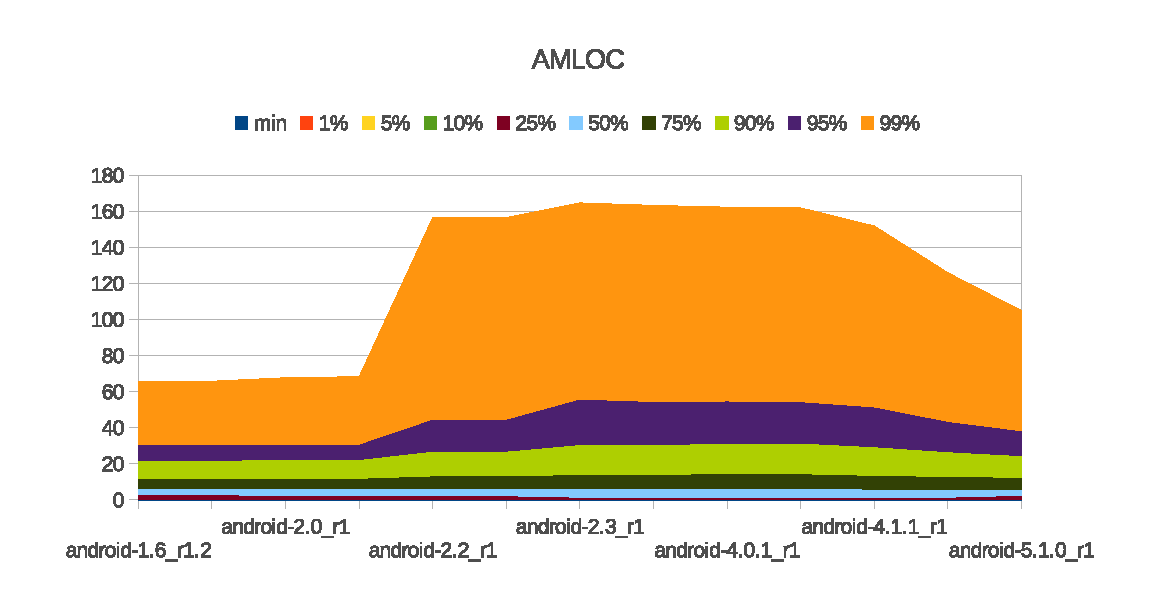
\includegraphics [keepaspectratio=true,scale=0.85]{figuras/graphs/amloc_android.eps}
\caption{Evolução da métrica AMLOC ao longo das versões da API}
\label{fig:amloc_android}
\end{figure}

A Tabela~\ref{tab:amloc_android} apresenta os valores para a métrica AMLOC nas versões do Android analisadas. É facilmente perceptível que a média de linhas de código por método não teve variação relevante. Em todas as versões analisadas, os valores muito frequentes, isto é, percentil 75, são métodos com até 14 linhas de código, enquanto de 14 a 30 aparecem como frequentes, e 31 a 55 pouco frequentes. A Figura~\ref{fig:amloc_android} apresenta a evolução da métrica AMLOC com a API, onde é possível ver uma variação muito pequena de valores para os percentis 75 e 90. O percentil 99 demonstra uma variação maior, mas ele representa dados não frequêntes na análise.

Esses são valores que estão de acordo com os apresentados em \citeonline{meirelles2013}, porém levemente menores para os percentis 75 e 90, com aproximadamente 3 linhas de código a menos por método. É possível perceber que os valores se mostraram bem semelhantes para o projeto Android, mesmo considerando o fato que este trabalho estuda apenas a API de desenvolvimento de aplicativos, essencialmente em Java e dentro do diretório ``\textit{frameworks}'' do AOSP, e \citeonline{meirelles2013} analiza todo o código fonte do sistema, que apresenta em sua totalidade uma maior proporção da linguagem C em relação as demais. Esses valores são subsídios para reafirmar que arquivos em C em geral, tem uma maior utilização de linhas de código do que arquivos em Java. \citeonline{oliveira2013} comenta que as diferenças entre as linguagems C/C++/Java para esta métrica não é significativa, uma vez que a sintaxe entre as 3 é bastante semelhante. Dada essa afirmação, podemos comparar os intervalos definidos por ele, chegando a conclusão de que os valores das métricas estão, para todas as versões, abaixo dos valores bom e regular para os percentis 75 e 90, o que é um bom resultado.

\begin{table}[!htb]
\centering
\scalefont{.7}
\begin{tabular}{|l|l|l|l|l|l|l|l|l|l|l|l|}
\hline
app&min&1\%&5\%&10\%&25\%&50\%&75\%&90\%&95\%&99\%&max\\
\hline
Launcher2&0&0&1&1&3&6.33333333333333&10.7797619047619&16.8961538461539&24.3825&48.3552380952381&57.5\\
\hline
Settings&0&0&0&0&3.625&8&15&21.46875&28.5&49.4&80.4166666666667\\
\hline
Camera2&0&0&0&0&1&4.5&9.85294117647059&16.0869565217391&21.5&38.28&66.6666666666667\\
\hline
Bluetooth&0&0&0&2.83068181818182&6.01923076923077&10.7928571428572&22.1571428571428&39.8633333333333&59.8399999999999&111.115&221\\
\hline
VoiceDialer&1&1.36&2.8&5&9.75&16&35.8333333333333&42.8&46.32&48.624&49.2\\
\hline
QuickSearchBox&0&0&1&1&3&4.38888888888889&6.16666666666667&10.5333333333334&13.15&22.28&32\\
\hline
Calculator&1&1&1&1&6.66666666666667&8.91666666666667&13.3333333333333&23.26&27.38&30.676&31.5\\
\hline
Mms&0&0&0&0&1&5.71428571428571&13.5210084033613&23.8111111111111&28.3464646464646&58.0447619047614&98\\
\hline
ManagedProvisioning&1&1&1&1&5.25&13.2833333333333&18.475&24.225&26.575&114.565&161\\
\hline
SoundRecorder&1&1.32&2.6&4.2&9&10&11.8&19.1472727272727&21.5963636363636&23.5556363636363&24.0454545454545\\
\hline
Terminal&0&0.15&0.75&1.84782608695652&3.09375&8.11904761904762&15.2916666666667&20.9166666666667&29.375&48.275&53\\
\hline
PackageInstaller&0&0.68&3.4&4&4.625&6.59444444444444&16.9833333333333&18.9&22.8882352941176&31.4482352941176&33.5882352941176\\
\hline
SpareParts&11&11.015&11.075&11.15&11.375&11.75&12.125&12.35&12.425&12.485&12.5\\
\hline
Tag&2&2.2275&3.1375&3.775&5&7.4&10.8333333333333&14.04&19.37&28.274&30.5\\
\hline
CertInstaller&1&1.2&2&3&3.85714285714285&6&9.96153846153845&16.15&20.7&24.34&25.25\\
\hline
KeyChain&0&0.51&2.55&3.35&5.5&8.2&12.875&23.1925&31.96875&52.7937499999999&58\\
\hline
Dialer&0&0&0&1&3&7&11.1300904977376&16.8928571428571&19.9793333333334&32.025&61.3333333333333\\
\hline
Browser&0&0&1&1&3.5&6.88588850174216&11&19&25.9478571428571&46.0230000000001&55.3333333333333\\
\hline
PhoneCommon&0&0.17&0.85&1&2.625&5.33333333333333&9.30128205128205&16.6270833333333&19.140625&27.428125&29.5\\
\hline
InCallUI&0&0&0&0&1&4.23333333333334&12&18.75&23.3153846153846&40.7666666666666&58\\
\hline
CellBroadcastReceiver&1&1.62&3.33&4.85&6.38333333333333&13.4285714285715&17.4488636363637&39.75&88.42&131.42&137\\
\hline
OneTimeInitializer&4&4.10666666666667&4.53333333333333&5.06666666666667&6.66666666666667&9.33333333333335&12&13.6&14.1333333333334&14.56&14.6666666666667\\
\hline
LegacyCamera&0&0&0&0.200000000000003&4&8.64285714285714&15.7777777777778&25.4666666666667&32.1799999999999&69.416&112.666666666667\\
\hline
Gallery2&0&0&0&0&3&6&11.5&17.3799019607843&21.6666666666667&44.3566666666666&107\\
\hline
BasicSmsReceiver&8.66666666666667&8.82666666666667&9.46666666666667&10.2666666666667&12.6666666666667&16.3333333333333&18.75&18.9&18.95&18.99&19\\
\hline
MusicFX&1&1.3&2.5&3&4.40476190476191&9.5851063829787&24&36.2149758454106&52.2391304347826&68.0478260869565&72\\
\hline
TvSettings&0&0&1&1&3.33333333333333&7&13.5&20.5214285714286&24.7208333333333&35.0591666666666&67\\
\hline
Stk&4.33333333333333&4.36&4.46666666666667&4.8&12&14.75&16.5&21.472&35.144&71.8288&81\\
\hline
UnifiedEmail&0&0&0&1&3&5&9.70833333333334&17&23.6666666666667&37.9499999999999&139.625\\
\hline
Launcher3&0&0&0&0&2.72727272727273&5.125&10.5862068965517&17.169696969697&24.79375&54.7072727272729&163.5\\
\hline
Music&0&0&0&1&4.1&9.51428571428572&16.890625&21.7578947368421&28.0010416666666&48.3157627118642&90\\
\hline
Camera&0&0&0&1&3&7.41666666666667&13&22.3742857142857&31.45&72.2308536585366&112.666666666667\\
\hline
Email&0&0&0&1&3.58333333333333&8&15.3484848484849&24.4866666666666&31.6104918032787&63.2823157894736&128\\
\hline
Nfc&0&0&0&1&3&9.64285714285714&18.5&31.6266666666667&38&42.48&70.5\\
\hline
Gallery&0&0.87&1&1&4&7.625&12.6733193277311&19.005&28.6&53.115&55\\
\hline
ContactsCommon&0&0&0&1&3.225&7.1&13&19&23.875&34.5000000000001&53.3333333333333\\
\hline
Contacts&0&0&0&1&3&6.45&11.5&18.61&23.721&63.535&86\\
\hline
DeskClock&0&0&0&1&5&9.15530303030303&15.2589285714286&24.02&27.2960558252427&30.7052380952381&40.1304347826087\\
\hline
FMRadio&0&0&0&0&0&0.5&11.7666504618376&20.0146666666667&32.125&70.355&96.5\\
\hline
\end{tabular}
\newline
\begin{tabular}{|l|l|l|l|l|l|l|l|l|l|l|l|}
\hline
HTMLViewer&5&5.12&5.6&6.2&8&11&14.5&16.6&17.3&17.86&18\\
\hline
Calendar&0&0&0&1&5&11.6666666666667&19.5833333333333&30.95&39.3&90&115.5\\
\hline
Exchange&0&0&0&1&4&10.0078431372549&17.3096153846154&28.4084615384616&34.6472222222222&44.405625&51.25\\
\hline
\end{tabular}

\caption{\textit{Average Method Lines of Code} nos aplicativos nativos}
\label{tab:amloc_apps}
\end{table}

Os valores apresentados na análise são relativamente baixos quando comparados com outros softwares livres, como demonstrado por \citeonline{meirelles2013}. Da mesma forma, quando olhamos os valores aplicativos do sistema, demonstrados na Tabela~\ref{tab:amloc_apps}, podemos perceber uma grande semelhança nos resultados. 

Métodos relacionados a interface gráfica tentem a ser relativamente grandes quando a interface é criada dinamicamente em Java, mas esse aumento não tem grande representatividade no código do sistema, uma vez que a maioria das partes do sistema que contém componentes gráficos estão nos aplicativos, como o launcher, settings e outros apps do sistema. Assim, aplicativos podem ter valores maiores de amloc, principalmente nos componentes do tipo \textit{Activity}.

Embora alguns poucos aplicativos tenham valores mais elevados para essa métrica, pode-se perceber que os intervalos se mantém válidos para a grande maioria dos aplicativos. Esses valores de aplicativos foram retirados dos aplicativos nativos da ultima versão do sistema analisada (Lollipop 5.1.0), e continuam se mantendo semelhantes ao sistema, como o próprio acoplamento à API sugere. 

Os aplicativos do sistema também se mantém dentro dos intervalos bom e regular definidos em \citeonline{oliveira2013}. Os valores para o percentil 95 também se encontram abaixo do valor regular, na maioria dos casos.

Em suma, os valores para os aplicativos se assemelham muito com os valores para as versões da API Android analisadas, levando então a conclusão de que os mesmos intervalos são válidos para as métricas em ambos os casos, embora se possa esperar valores menores em aplicativos, porém com uma maior variância. Essa variância se dá pelo diferente propósito de cada aplicativo, que utiliza pedaços variados do sistema e tem sua codificação adaptada para seu propósito.

Intervalos encontrados:

\begin{itemize}
\item Valores abaixo de 14 se mostraram muito frequentes para os aplicativos e para a API;
\item Enquanto no sistema os valores para o percentil 90 se encontram abaixo de 31, nos aplicativos eles alcançam em poucos casos, ficando em sua maioria abaixo de 25;
\item Valores acima de 31 são pouco frequentes em ambos os casos;
\end{itemize}

\subsection{Average Cyclomatic Complexity per Method}

\begin{figure}[!htb]
\centering
\includegraphics [keepaspectratio=true,scale=0.85]{figuras/graphs/accm_android.eps}
\caption{Evolução da métrica ACCM ao longo das versões da API}
\label{fig:accm_android}
\end{figure}

A Figura~\ref{fig:accm_android} apresenta a evolução de ACCM métrica com a evolução da API. Podemos perceber que essa métrica não teve uma variação grande ao longo das versões nos percentis 75, 90 e 95, e o pouco do valor que ganhou nas versões centrais do gráfico foi sendo novamente reduzido nas versões seguintes. Valores sinalizados com 0 ocorrem em classes que não contém métodos.

\begin{table}[!htb]
\centering
\scalefont{.7}
\begin{tabular}{|l|l|l|l|l|l|l|l|l|l|l|l|l|}
\hline
version&classes&min&1\%&5\%&10\%&25\%&50\%&75\%&90\%&95\%&99\%&max\\
\hline
android-1.6\_r1.2&5745&0&0&0&0&1&1.11111111111111&2&3.45454545454545&4.68831967213114&9.5&55\\
\hline
android-1.6\_r1.5&5745&0&0&0&0&1&1.11111111111111&2&3.45454545454545&4.68831967213114&9.5&55\\
\hline
android-2.0\_r1&6331&0&0&0&0&1&1.11111111111111&2&3.5&4.75&9.74444444444443&59\\
\hline
android-2.1\_r2.1p2&6360&0&0&0&0&1&1.11882352941176&2&3.5&4.8&9.88199999999997&60\\
\hline
android-2.2\_r1&7352&0&0&0&0&1&1.06666666666667&2&3.73840579710146&5.2752380952381&12&99\\
\hline
android-2.2.3\_r2&7358&0&0&0&0&1&1.06666666666667&2.01744186046512&3.75&5.26173913043478&12&99\\
\hline
android-2.3\_r1&8093&0&0&0&0&1&1&2.07142857142857&4&5.81691176470588&12.8275&99\\
\hline
android-2.3.7\_r1&8240&0&0&0&0&1&1&2.08333333333333&4&5.8&12.755625&99\\
\hline
android-4.0.1\_r1&11709&0&0&0&0&1&1&2.125&4&6&17&94.3333333333333\\
\hline
android-4.0.4\_r2.1&11851&0&0&0&0&1&1&2.10858585858586&4&6&17&94.3333333333333\\
\hline
android-4.1.1\_r1&14115&0&0&0&0&1&1&2&3.85631469979296&5.77846153846152&16&99.4\\
\hline
android-5.1.0\_r1&20129&0&0&0&0&1&1&2&3.5&5&11&158.6\\
\hline
\end{tabular}

\caption{\textit{Average Cyclomatic Complexity per Method} no Android}
\label{tab:accm_android}
\end{table}

\begin{figure}[!htb]
\centering
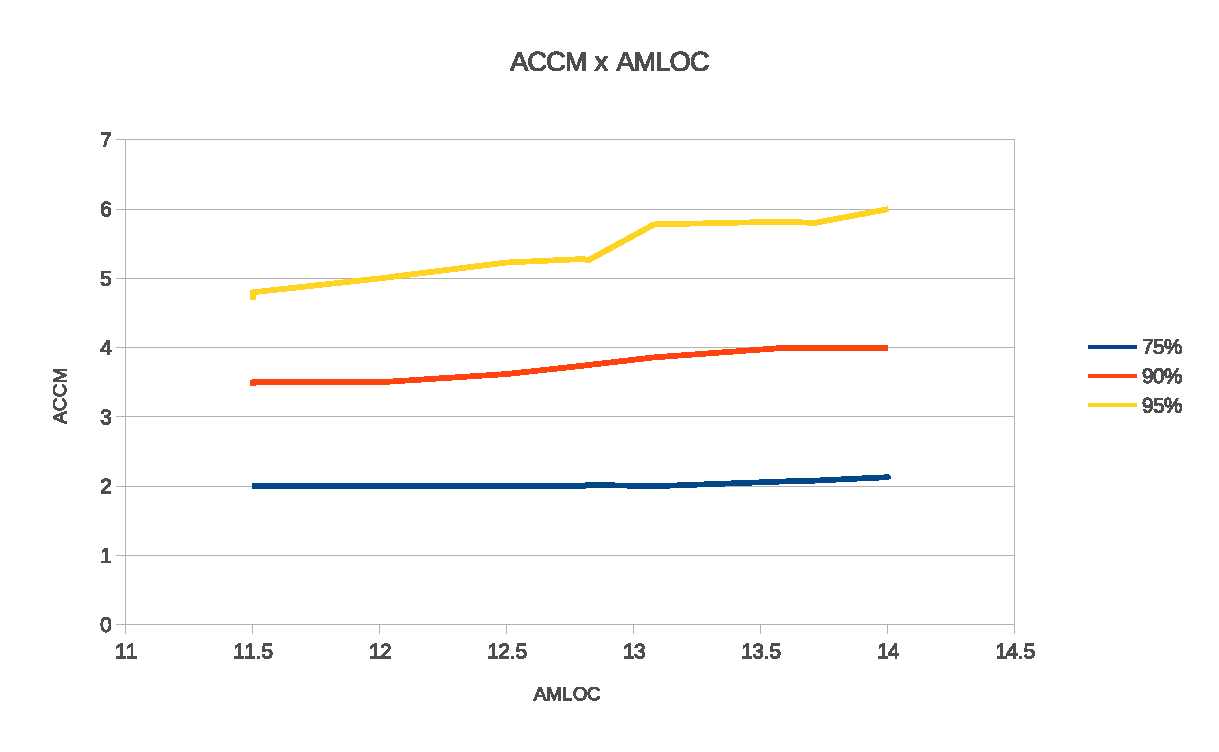
\includegraphics [keepaspectratio=true,scale=0.85]{figuras/ACCMxAMLOC.eps}
\caption{ACCM por AMLOC nas Tabelas~\ref{tab:amloc_android} e~\ref{tab:accm_android}}
\label{fig:accmxamloc}
\end{figure}

Uma relação entre ACCM e AMLOC pode ser claramente vista na Tabela~\ref{tab:accm_android} e está melhor demonstrada no gráfico da Figura~\ref{fig:accmxamloc}. Nos valores do percentil 75, que correspondem a valores muito frequentes, as versões de 2.2.3 a 4.0.4 contém os únicos valores para o sistema onde a complexidade ciclomática supera o número 2, e não por acaso são os valores com maior AMLOC nesse percentil como pode ser visto na Tabela~\ref{tab:amloc_android}. Essa relação direta também pode ser vista nos percentis 90 e 95, que representam valores frequentes e pouco requentes, respectivamente.

\begin{table}[!htb]
\centering
\scalefont{.7}
\documentclass[a4paper]{article}
\usepackage[T1]{fontenc}
\usepackage[latin1]{inputenc}
\begin{document}
\begin{tabular}{|l|l|l|l|l|l|l|l|l|l|l|l|}
\hline
app&min&1\%&5\%&10\%&25\%&50\%&75\%&90\%&95\%&99\%&max\\
\hline
Launcher2&0&0&1&1&1&1.4&2.09318181818182&3&3.61545454545454&8.67642857142855&11.8666666666667\\
\hline
Settings&0&0&0&0&1&1.57142857142857&2.5&3.66666666666667&4.42857142857143&8&17\\
\hline
Camera2&0&0&0&0&1&1&1.83333333333333&2.66666666666667&3.5&6&8.3\\
\hline
Bluetooth&0&0&0&1&1.33333333333333&2.19337979094077&4&7.95&10.3625&24.2866666666666&49\\
\hline
VoiceDialer&1&1&1&1&1.75&3.5&6.16666666666667&8.52&8.93999999999999&11.388&12\\
\hline
QuickSearchBox&0&0&1&1&1&1.03333333333333&1.66666666666667&2.47142857142857&3&4.67666666666667&5\\
\hline
Calculator&1&1&1&1&1.33333333333333&1.58333333333333&2.66666666666667&3.53333333333333&5.26666666666667&6.65333333333333&7\\
\hline
Mms&0&0&0&0&1&1.28571428571429&2.43650793650793&3.55555555555556&5.4125&10.2285714285714&16\\
\hline
ManagedProvisioning&1&1&1&1&1&2.16764705882353&2.98076923076923&3.24&3.575&5.26000000000001&6\\
\hline
SoundRecorder&1&1.01714285714286&1.08571428571429&1.17142857142857&1.42857142857143&1.6&1.9047619047619&2.94372294372294&3.29004329004329&3.56709956709957&3.63636363636364\\
\hline
Terminal&0&0.15&0.75&1&1&1.5&1.73809523809524&4.8&8.25&10.45&11\\
\hline
PackageInstaller&0&0.17&0.85&1&1&1.2984126984127&2.86458333333333&3.7&4.07058823529412&4.39058823529412&4.47058823529412\\
\hline
SpareParts&1&1.01357142857143&1.06785714285714&1.13571428571429&1.33928571428571&1.67857142857143&2.01785714285715&2.22142857142857&2.28928571428572&2.34357142857143&2.35714285714286\\
\hline
Tag&1&1&1&1&1.1&1.6&1.95833333333334&2.71666666666667&2.975&3.395&3.5\\
\hline
CertInstaller&1&1&1&1&1&1.57142857142857&2.40384615384616&2.7&3.35&3.87&4\\
\hline
KeyChain&0&0.17&0.85&1&1.08333333333333&1.66666666666667&2&2.73&3.51875&3.60375&3.625\\
\hline
Dialer&0&0&0&1&1&1.16666666666667&2&2.77142857142857&3&3.9675&57.8333333333333\\
\hline
Browser&0&0&1&1&1&1.5&2.16666666666667&3.26896551724138&4.03749999999999&7.02500000000001&8.8\\
\hline
PhoneCommon&0&0.17&0.85&1&1&1.16666666666666&1.75&3.51666666666667&5.6125&6.1225&6.25\\
\hline
InCallUI&0&0&0&0&1&1.05555555555555&2.00595238095238&2.76318681318681&4&6.69999999999999&8.33333333333333\\
\hline
CellBroadcastReceiver&1&1&1&1&1.2390350877193&1.76623376623377&3.33928571428572&6.13&9.72&13.636&15\\
\hline
OneTimeInitializer&1&1.02&1.1&1.2&1.5&2&2.5&2.8&2.9&2.98&3\\
\hline
LegacyCamera&0&0&0&0.200000000000003&1&1.6&2.39655172413793&3.36666666666667&4.10599078341013&9.58666666666667&10\\
\hline
Gallery2&0&0&0&0&1&1.375&2.16176470588236&3&3.705&6.01399999999999&11\\
\hline
BasicSmsReceiver&1.33333333333333&1.34333333333333&1.38333333333333&1.43333333333333&1.58333333333334&1.70833333333334&1.99431818181818&2.43409090909091&2.58068181818182&2.69795454545455&2.72727272727273\\
\hline
MusicFX&1&1&1&1&1&2&3.13166666666667&4.96521739130435&7.09782608695653&9.4195652173913&10\\
\hline
TvSettings&0&0&1&1&1&1.40689655172414&2.48026315789474&3.77417582417583&4.7125&6.39749999999998&12\\
\hline
Stk&1&1&1&1.2&2&2.5&3.5&4.724&7.09999999999999&13.82&15.5\\
\hline
UnifiedEmail&0&0&0&1&1&1.16666666666667&1.93541666666667&2.83333333333333&3.66666666666667&6.69166666666666&53\\
\hline
Launcher3&0&0&0&0&1&1.23076923076923&2&3&4&9.87212121212122&30\\
\hline
Music&0&0&0&1&1&1.66666666666667&2.5&3.37436440677966&4.31484517304189&8.96624999999995&18\\
\hline
Camera&0&0&0&1&1&1.49418604651163&2.26559829059829&3.16944801026957&3.96642857142857&9.83000000000001&17\\
\hline
Email&0&0&0&1&1&1.33333333333333&2&3.02222222222222&4.17721139430285&7.50999999999999&19.4\\
\hline
Nfc&0&0&0&1&1&2&3.35294117647059&5.16140350877193&7.86666666666666&9.62&15.5\\
\hline
Gallery&0&0.87&1&1&1&1.6125&2.5&3.35333333333333&3.9125&7.25999999999999&9\\
\hline
ContactsCommon&0&0&0&1&1&1.28571428571429&2&3.44444444444444&4.54166666666667&7&7.5\\
\hline
Contacts&0&0&0&1&1&1.23214285714285&2&3&3.64017857142857&9.74000000000001&21\\
\hline
DeskClock&0&0&0&1&1&1.6875&2.28928571428572&3.25833333333333&3.81&4.48642857142857&5.33333333333333\\
\hline
FMRadio&0&0&0&0&0&0.5&1.69602272727273&2.535&3.27298850574712&9.76500000000001&13.5\\
\hline
\end{tabular}
\newline
\begin{tabular}{|l|l|l|l|l|l|l|l|l|l|l|l|}
\hline
HTMLViewer&1.5&1.51&1.55&1.6&1.75&2&2&2&2&2&2\\
\hline
Calendar&0&0&0&1&1&2&3&4.68&6.325&14.93&19\\
\hline
Exchange&0&0&0&1&1&1.65526315789473&3.2&4.49&5.4112443778111&6.82623913043478&7.66666666666667\\
\hline
\end{tabular}
\end{document}

\caption{\textit{Average Cyclomatic Complexity per Method} nos aplicativos nativos}
\label{tab:accm_apps}
\end{table}

Essa relação pode ser vista para os aplicativos. Embora não seja totalmente determinístico, no geral aplicativos com maiores valores de AMLOC tendem a ter um maior valor de ACCM, assim como visto na API do sistema. Com exceção do \textit{SMSReceiver}, os 5 aplicativos com maior valor de AMLOC são os que contém maior complexidade do conjunto. 

Reforçando a importância dessa métrica em uma análise estática de código, \citeonline{oliveira2013} define a mesma com um peso adicional em relação a outras métricas em seu estudo. Valores de referência definidos para esse estudo foram 1 a 3, 3 a 5, e 5 a 7, para excelente, bom e regular, respectivamente. Observando as Tabelas~\ref{tab:accm_android} e~\ref{tab:accm_apps} percebe-se que os valores obtidos neste trabalho estão dentro do intervalo excelente ou bom, para os percentis 75 e 90, e dentro de bom ou regular para o percentil 95, que representa valores menos frequentes. No geral, os resultados indicam que o sistema tem uma boa complexidade ciclomática e que os aplicativos desenvolvidos para o mesmo acompanham essa mesma linha. \citeonline{meirelles2013} definiu intervalos semelhantes para códigos em C, e valores um pouco reduzidos para códigos em C++ e Java (0 a 2, 2 a 4, e 4 a 6 para os percentis 75, 90 e 95 respectivamente).  Os resultados encontrados para a API do sistema Android se encontram todos dentro desses intervalos, confirmando como um bom resultado. Já os aplicativos tem algumas exceções que extrapolam levemente esses valores, mas continuam em sua maioria dentro desses limites.

Baseando-se nessas observações, são considerados os seguintes intervalos:

\begin{itemize}
\item Valores abaixo 2 se mostraram muito frequentes para os aplicativos e para a API, e até 2.5 são considerados excelentes. É importante relembrar que uma complexidade ciclomática 2 implica em afirmar que 2 testes unitários resultam em 100\% de cobertura para esse trecho de código;
\item ACCM menor ou igual a 4 pode ser vista em todas as versões do Android e na grande maioria dos aplicativos dentro do percentil 90, sendo uma referência para um valor maior mas ainda considerado bom. Os aplicativos do sistema quase não alcançaram esse valor;
\item Valores acima de 4 são considerados regulares e são pouco frequentes em ambos os casos, porém para a API do sistema o percentil 95 chegou a 6. Valores acima de 6 são bem raros e correspondem a uma quantidade estatisticamente desprezível para esta análise.
\end{itemize}

\subsection{Response For a Class}

\begin{table}[!htb]
\centering
\scalefont{.7}
\begin{tabular}{|l|l|l|l|l|l|l|l|l|l|l|l|l|}
\hline
version&classes&min&1\%&5\%&10\%&25\%&50\%&75\%&90\%&95\%&99\%&max\\
\hline
android-1.6\_r1.2&5745&0&0&0&0&2&10&31&79&133.8&357.480000000003&2858\\
\hline
android-1.6\_r1.5&5745&0&0&0&0&2&10&31&79&133.8&357.480000000003&2858\\
\hline
android-2.0\_r1&6331&0&0&0&0&2&10&31&79&131.5&350&2902\\
\hline
android-2.1\_r2.1p2&6360&0&0&0&0&2&10&32&79&133.049999999999&352.869999999999&2923\\
\hline
android-2.2\_r1&7352&0&0&0&0&2&9&30&77.9000000000005&131.45&372.449999999999&2754\\
\hline
android-2.2.3\_r2&7358&0&0&0&0&2&9&30&78&131.15&372.150000000001&2754\\
\hline
android-2.3\_r1&8093&0&0&0&0&1&8&27&76&129&358&2347\\
\hline
android-2.3.7\_r1&8240&0&0&0&0&1&8&27&76&130&354.219999999999&2347\\
\hline
android-4.0.1\_r1&11709&0&0&0&0&1&7&28&82&140&388&2871\\
\hline
android-4.0.4\_r2.1&11851&0&0&0&0&1&7&28&81&141&391&2921\\
\hline
android-4.1.1\_r1&14115&0&0&0&0&1&7&26&77.6000000000004&136&363.720000000001&6596\\
\hline
android-5.1.0\_r1&20129&0&0&0&0&2&9&30&84&156&775.720000000001&11010\\
\hline
\end{tabular}

\caption{\textit{Response For a Class} no Android}
\label{tab:rfc_android}
\end{table}

A API do sistema Android tende a ter um valor relativamente alto de RFC devido a forma como sua arquitetura foi desenhada, como pode ser visto na Tabela~\ref{tab:rfc_android}. Serviços do sistema são acessados muitas vezes através de objetos do sistema, e para seu uso correto alguns métodos devem ser chamados explicitamente. Por exemplo, para acessar o \textit{bluetooth}, não se chama diretamente um método de uma classe \textit{BluetoothAdapter}, pois os serviços do sistema geralmente estão encapsulados e são retornados por um método \textit{get()}, seguidos dos métodos que se deseja utilizar desse serviço. Por exemplo, para verificar dispositivos \textit{bluetooth} próximos, deve-se obter o \textit{adapter} via chamada estática de método para a própria classe para obter a instância, seguida de uma chamada de método para início de \textit{discovery} de dispositivos, e em seguida utilizar os métodos \textit{isDiscoverying()} e \textit{cancelDiscovery()} para controlar a busca. Um acesso direto a uma variável booleana removeria a necessidade da chamada de método \textit{isDiscoverying()}, entretanto perderia seu encapsulamento. De forma geral, encapsulamento de variáveis tende a aumentar o valor de RFC, que conta apenas métodos. 

\begin{figure}[!htb]
\centering
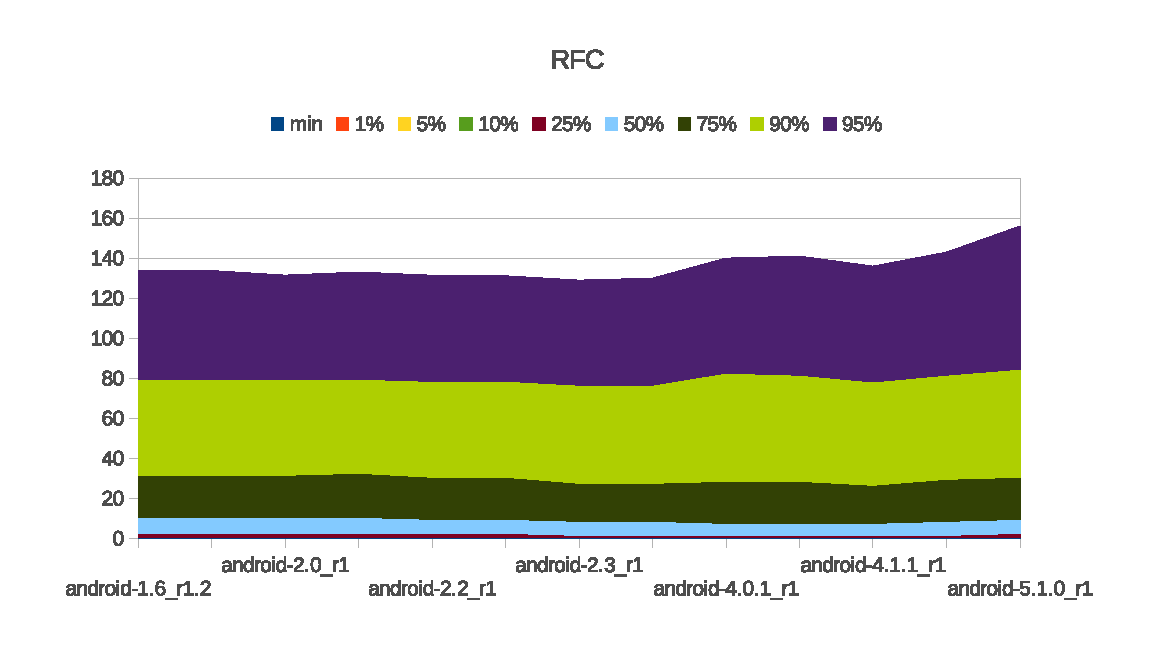
\includegraphics [keepaspectratio=true,scale=0.85]{figuras/graphs/rfc_android.eps}
\caption{Evolução da métrica RFC ao longo das versões da API}
\label{fig:rfc_android}
\end{figure}

Contribuindo para o aumento, o resultado da busca de dispositivos bluetooth é realizado de forma assíncrona na forma de mensagens utilizando \textit{intents} (vide Capítulo~\ref{cap:android-os}), então mais um método é criado dentro de um \textit{receiver} (que pode ser a própria classe estendendo \textit{BroadcastReceiver}) para receber essa mensagem, aumentando um pouco o valor de RFC. Uma comunicação síncrona hipotética com uma chamada estática direta como \textit{BluetoothAdapter.discoverNearDevices()} retornando uma lista seria em teoria uma forma muito mais simples de ser utilizada, porém perderia a proteção do encapsulamento e deixaria de utilizar o comportamento em escopo de objeto para usar em escopo de classe, e também se perderia o maior controle sobre a própria busca que a API dá ao usuário com os métodos adicionais. Além disso, o encapsulamento de serviço dos sistema é um controle adicional que permite que o mesmo escalone melhor a utilização de recursos que necessitem de exclusão mútua. Por exemplo, um acesso direto a câmera dificultaria o sistema de dar acesso a 1 cliente de cada vez, pois afinal, o usuário não consegue usar a câmera, por exemplo, em dois aplicativos simultaneamente.

Comunicações assíncronas são muito usadas ao longo de todo o sistema para utilização de recursos, e então é necessário ter uma forma de receber mensagens de aplicativos e do sistema, o que é feito com a classe \textit{BroadcastReceiver} e implementando métodos específicos da mesma. Mesmo fora do contexto Android, comunicações assíncronas tendem a criar métodos adicionais de comunicação, como é visto no padrão \textit{Observer}, que se assemelha muito a essa comunicação por \textit{Intents}. A Figura~\ref{fig:rfc_android} demonstra que essa métrica não teve variação grande ao longo das versões do Android, tendendo inclusive a um leve aumento nas ultimas versões, demonstrando que os valores altos apresentados são mesmo uma característica da arquitetura do sistema. 

\begin{table}[!htb]
\centering
\scalefont{.7}
\begin{tabular}{|l|l|l|l|l|l|l|l|l|l|l|l|}
\hline
app&min&1\%&5\%&10\%&25\%&50\%&75\%&90\%&95\%&99\%&max\\
\hline
Launcher2&0&0&1&1&3.75&12.5&37.25&84.4&178.75&850.719999999999&1061\\
\hline
Settings&0&0&0&0&3&10&31&69&112&229.2&596\\
\hline
Camera2&0&0&0&0&1&6&22&65&113&352.199999999998&752\\
\hline
Bluetooth&0&0&0&2&8&25&68.75&131.3&205.6&468.34&658\\
\hline
VoiceDialer&2&2&2&2&6&14&37&59.4&87.8999999999999&137.58&150\\
\hline
QuickSearchBox&0&0&1&1&3&8&19&30&57.3&115.12&213\\
\hline
Calculator&1&1&1&1&6&8&13&42.8&62.4&78.08&82\\
\hline
Mms&0&0&0&0&2&10&30.5&76.6&122&247.36&788\\
\hline
ManagedProvisioning&1&1&1.85&2&2.25&7.5&49.5&66.4&80.2&93.3&97\\
\hline
SoundRecorder&2&2.84&6.2&10.4&23&28&94&130.6&142.8&152.56&155\\
\hline
Terminal&0&0.15&0.75&1&3&13&47.5&52.5&56.5&64.9&67\\
\hline
PackageInstaller&0&0.17&0.85&2.4&3&10.5&26&62.5000000000001&128&155.2&162\\
\hline
SpareParts&1&1.6&4&7.00000000000001&16&31&46&55&58&60.4&61\\
\hline
Tag&1&1.14&1.7&2.4&4&9&16&20.2&25.5&33.9&36\\
\hline
CertInstaller&1&1&1&1&3.5&6&14.5&86&109.5&128.3&133\\
\hline
KeyChain&0&0.17&0.85&1.7&4&9.5&13.75&21.1&26.3&27.66&28\\
\hline
Dialer&0&0&0&1&3&8.5&25&66.4&113.1&250.74&321\\
\hline
Browser&0&0&1&1&3.25&13&36.75&78.6&124.35&328.89&795\\
\hline
PhoneCommon&0&0.17&0.85&1&3&5.5&9&30.8&43.95&52.79&55\\
\hline
InCallUI&0&0&0&0&1&8&28.25&82.5&120.25&297.349999999999&434\\
\hline
CellBroadcastReceiver&1&1&1&2&5&15.5&26&33.4&54.8&75.63&84\\
\hline
OneTimeInitializer&2&2.18&2.9&3.8&6.5&11&15.5&18.2&19.1&19.82&20\\
\hline
LegacyCamera&0&0&0&0.200000000000003&3&11&38&77.6&139.6&400.76&742\\
\hline
Gallery2&0&0&0&0&3&12&33.75&77.7&110&312.14&595\\
\hline
BasicSmsReceiver&7&7.03&7.15&7.3&7.75&12.5&24.75&38.7&43.35&47.07&48\\
\hline
MusicFX&1&1&1&1.5&2.75&5.5&35.25&125&147.5&194.3&206\\
\hline
TvSettings&0&0&1&1&3&14&41&76.9&107.65&191.599999999999&775\\
\hline
Stk&1&1.16&1.8&2.6&6&18&45&125.6&179.2&304.64&336\\
\hline
UnifiedEmail&0&0&0&1&3&9&25&59&114.5&356.8&1012\\
\hline
Launcher3&0&0&0&0&2&9&31&77.8&144.6&515.640000000001&1407\\
\hline
Music&0&0&0&1&2&6.5&19.75&45.6000000000001&94.9999999999999&155.5&192\\
\hline
Camera&0&0&0&1&2&10&33&80&128.5&307.27&921\\
\hline
Email&0&0&0&1&2.5&9&28&60&93.1999999999999&192.22&399\\
\hline
Nfc&0&0&0&1&3&16&37&93.8&155&263.44&306\\
\hline
Gallery&0&0.87&1&1&4&17&31.5&68.3&118.7&224.66&296\\
\hline
ContactsCommon&0&0&0&1&3&9&22&60&105.5&199.4&271\\
\hline
Contacts&0&0&0&1&3&8.5&23&59&96.25&253.46&463\\
\hline
DeskClock&0&0&0&1&4.75&21&50.25&121.3&151.35&230.25&691\\
\hline
FMRadio&0&0&0&0&0&0.5&18.25&75.4&105.85&277.05&414\\
\hline
\end{tabular}
\newline
\begin{tabular}{|l|l|l|l|l|l|l|l|l|l|l|l|}
\hline
HTMLViewer&1&1.06&1.3&1.6&2.5&4&4.5&4.8&4.9&4.98&5\\
\hline
Calendar&0&0&0&1&4&13&37.5&109.6&160&422.799999999998&1291\\
\hline
Exchange&0&0&0&1&4&14&37.75&72.1&107.55&162.05&224\\
\hline
\end{tabular}

\caption{\textit{Response For a Class} nos aplicativos nativos}
\label{tab:rfc_apps}
\end{table}


Em suma, na API do sistema, o valor de RFC pode ser considerado alto, porém justificável. Os componentes do Android podem ter seu valor RFC e DIT mais alto que outras classes em Java devido ao nível de herança que eles apresentam. Por exemplo, um componente gráfico em um \textit{app} herda de \textit{Activity}, que por sua vez herda de \textit{Context}, que contém uma estrutura de hierarquia intermediária.

O acoplamento entre a própria API de desenvolvimento e o aplicativos fica exemplificado com o valor dessa métrica sendo alto para ambos os casos. É importante lembrar que componentes do sistema se comunicam da mesma forma com outros componentes do sistema como se comunicam com aplicativos desenvolvidos para o mesmo. A Tabela~\ref{tab:rfc_apps} demonstra os valores de RFC para aplicativos nativos.

\citeonline{meirelles2013} define como bons intervalos para projetos Java valores de 0 a 9, 10 a 26, e 27 a 59, para os percentis 75, 90 e 95, respectivamente. Pode-ses perceber que os valores na análise da API obtidos neste trabalho estão bem acima desse valor, estando em seu percentil 75 um valor perto de 30, que seria no máximo regular nessa escala.

Baseando-se em todas essas observações, são considerados os seguintes intervalos:

\begin{itemize}
\item Valores abaixo 31 se mostraram muito frequentes para API Android. Para os aplicativos do sistema, existe uma grande variância de valores, porém estando em sua grande maioria abaixo de 38 para o percentil 75.
\item RFC chegou a 130 em aplicativos nativos, porém no geral não alcançam o valor 85. Esse mesmo valor é o limite para a API do sistema.
\item Valores acima de 85 são valores considerados altos para a métrica RFC, e são pouco frequentes nos dados analisados. Valores acima de 140 não são frequentes.
\end{itemize}

Um intervalo de valores até 38 pode ser considerado bom para aplicativos, e regular no intervalo desse valor até o 85. Acima disso são considerados valores altos, mas parecem ser comuns no Android, então são aceitáveis. Esses intervalos aqui encontrados estão mais próximos dos limites definidos por \citeonline{meirelles2013} para a Linguagem C do que para Java. Inclusive os valores aqui encontrados aqui para a API Android, essencialmente em Java, se mostram bastante semelhantes aos valores para o projeto Android como um todo, com predominância da linguagem C, encontrados por \citeonline{meirelles2013}. Essa semelhança pode levar a interpretação de que estilos semelhantes de estruturação e design são utilizados em todo o AOSP, independente da linguagem utilizada em cada módulo.

\subsection{Depth of Inheritance Tree / Number of Children}

\begin{figure}[!htb]
\centering
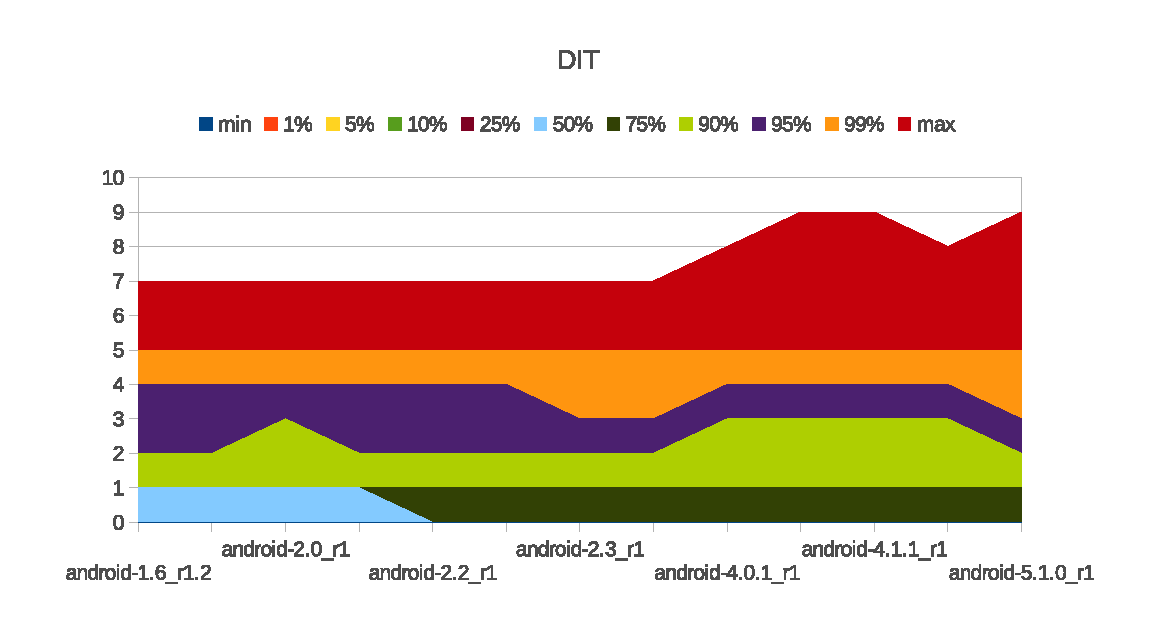
\includegraphics [keepaspectratio=true,scale=0.85]{figuras/graphs/dit_android.eps}
\caption{Evolução da métrica DIT ao longo das versões da API}
\label{fig:dit_android}
\end{figure}

\begin{figure}[!htb]
\centering
\includegraphics [keepaspectratio=true,scale=0.85]{figuras/graphs/noc_android.eps}
\caption{Evolução da métrica NOC ao longo das versões da API}
\label{fig:noc_android}
\end{figure}

As Figuras~\ref{fig:dit_android} e~\ref{fig:noc_android} demonstram o comportamento dessas métricas com a evolução do sistema. É possível perceber que são valores relativamente baixos e com variação muito pequena para as duas métricas. Para DIT podemos perceber que os valores para cada percentil varia em no máximo 1 em algumas versões e depois voltam ao valor anterior. NOC também se mantém 0 ou 1 para o percentil 90 em todas as versões.

\begin{table}[!htb]
\centering
\scalefont{.7}
\begin{tabular}{|l|l|l|l|l|l|l|l|l|l|l|l|l|}
\hline
version&classes&min&1\%&5\%&10\%&25\%&50\%&75\%&90\%&95\%&99\%&max\\
\hline
android-1.6\_r1.2&5745&0&0&0&0&0&1&1&2&4&5&7\\
\hline
android-1.6\_r1.5&5745&0&0&0&0&0&1&1&2&4&5&7\\
\hline
android-2.0\_r1&6331&0&0&0&0&0&1&1&3&4&5&7\\
\hline
android-2.1\_r2.1p2&6360&0&0&0&0&0&1&1&2&4&5&7\\
\hline
android-2.2\_r1&7352&0&0&0&0&0&0&1&2&4&5&7\\
\hline
android-2.2.3\_r2&7358&0&0&0&0&0&0&1&2&4&5&7\\
\hline
android-2.3\_r1&8093&0&0&0&0&0&0&1&2&3&5&7\\
\hline
android-2.3.7\_r1&8240&0&0&0&0&0&0&1&2&3&5&7\\
\hline
android-4.0.1\_r1&11709&0&0&0&0&0&0&1&3&4&5&8\\
\hline
android-4.0.4\_r2.1&11851&0&0&0&0&0&0&1&3&4&5&9\\
\hline
android-4.1.1\_r1&14115&0&0&0&0&0&0&1&3&4&5&9\\
\hline
android-4.3.1\_r1&15472&0&0&0&0&0&0&1&3&4&5&8\\
\hline
android-5.1.0\_r1&20129&0&0&0&0&0&0&1&2&3&5&9\\
\hline
\end{tabular}

\caption{\textit{Depth of Inheritance Tree} no Android}
\label{tab:dit_android}
\end{table}

\begin{table}[!htb]
\centering
\scalefont{.7}
\documentclass[a4paper]{article}
\usepackage[T1]{fontenc}
\usepackage[latin1]{inputenc}
\begin{document}
\begin{tabular}{|l|l|l|l|l|l|l|l|l|l|l|l|}
\hline
app&min&1\%&5\%&10\%&25\%&50\%&75\%&90\%&95\%&99\%&max\\
\hline
Launcher2&0&0&0&0&0&1&1&1&2&2.41&3\\
\hline
Settings&0&0&0&0&0&1&2&2&2&3&4\\
\hline
Camera2&0&0&0&0&0&0&1&1&2&3&3\\
\hline
Bluetooth&0&0&0&0&0&0&1&1&2&2&2\\
\hline
VoiceDialer&0&0&0&0&0&0&1&1&1&1&1\\
\hline
QuickSearchBox&0&0&0&0&0&1&1&2&3&5&5\\
\hline
Calculator&0&0&0&0&0&1&1&1&1&1&1\\
\hline
Mms&0&0&0&0&0&1&1&2&3&4&6\\
\hline
ManagedProvisioning&0&0&0&0&0&0&1&1&1&1&1\\
\hline
SoundRecorder&0&0&0&0&0&1&1&1&1&1&1\\
\hline
Terminal&0&0&0&0&0&0&1&1&1&1&1\\
\hline
PackageInstaller&0&0&0&0&0&1&1&1&1&1&1\\
\hline
SpareParts&1&1&1&1&1&1&1&1&1&1&1\\
\hline
Tag&0&0&0&0&0&1&1&1&1&1&1\\
\hline
CertInstaller&0&0&0&0&0.5&1&1.5&2&2&2&2\\
\hline
KeyChain&0&0.17&0.85&1&1&1&1&1&1&1&1\\
\hline
Dialer&0&0&0&0&0&0.5&1&1&1&2&2\\
\hline
Browser&0&0&0&0&0&1&1&1&2&2&2\\
\hline
PhoneCommon&0&0&0&0&0&0&1&1&1.15&1.83&2\\
\hline
InCallUI&0&0&0&0&0&0&1&1&2&2&2\\
\hline
CellBroadcastReceiver&0&0&0&0&1&1&1&1&1.45&2&2\\
\hline
OneTimeInitializer&1&1&1&1&1&1&1&1&1&1&1\\
\hline
LegacyCamera&0&0&0&0&0&0&1&2&2&3&4\\
\hline
Gallery2&0&0&0&0&0&1&1&2&2&3&4\\
\hline
BasicSmsReceiver&1&1&1&1&1&1&1&1&1&1&1\\
\hline
MusicFX&0&0&0&0&0&1&1&1.5&2.25&2.85&3\\
\hline
TvSettings&0&0&0&0&0&1&1&2&3&4&4\\
\hline
Stk&0&0&0&0&1&1&1&1&1&1&1\\
\hline
UnifiedEmail&0&0&0&0&0&1&1&2&2&3&4\\
\hline
Launcher3&0&0&0&0&0&1&1&1&2&3&3\\
\hline
Music&0&0&0&0&0&1&1&1&1&1&1\\
\hline
Camera&0&0&0&0&0&0&1&1&2&3&3\\
\hline
Email&0&0&0&0&0&1&1&1&2&2&3\\
\hline
Nfc&0&0&0&0&0&0&1&1&1&1&1\\
\hline
Gallery&0&0&0&0&0&1&1&2&2&3&3\\
\hline
ContactsCommon&0&0&0&0&0&1&1&1&2&3.10000000000002&5\\
\hline
Contacts&0&0&0&0&0&1&1&1&2&2&3\\
\hline
DeskClock&0&0&0&0&0&1&1&2&2&3&3\\
\hline
FMRadio&0&0&0&0&0&0&1&1&1&1&1\\
\hline
\end{tabular}
\newline
\begin{tabular}{|l|l|l|l|l|l|l|l|l|l|l|l|}
\hline
HTMLViewer&1&1&1&1&1&1&1&1&1&1&1\\
\hline
Calendar&0&0&0&0&0&1&1&1&2&2&2\\
\hline
Exchange&0&0&0&0&0&1&1&1&2&2&2\\
\hline
\end{tabular}
\end{document}

\caption{\textit{Depth of Inheritance Tree} nos aplicativos nativos}
\label{tab:dit_apps}
\end{table}

A primeira observação sobre o dados das Tabelas~\ref{tab:dit_android} e~\ref{tab:dit_apps} é que elas contém um número grande de zeros até o percentil 50. Como a linguagem Java representa mais de 85\% da amostra, vários desses zeros estão presentes também na linguagem Java. O que tiramos disso é que a ferramenta Analizo não contabiliza a classe Object na métrica DIT, pois caso contabilizasse o valor mínimo para o Java seria 1, visto que todo objeto Java herda de Object. Tirando esse fato não temos muitas surpresas, os valores são em geral baixos, chegando a no máximo 4 até o percentil 95 em todos as versões da API, demonstrando valores bem menores dos que os intervalos definidos por \citeonline{meirelles2013} para Java, que chegam até 2, 4 e 6 para os percentis 75, 90 e 95, respectivamente. \citeonline{oliveira2013} utiliza os mesmos intervalos para excelente, bom, e regular, respectivamente. \citeonline{ferreira2009} não define intervalos para essa métrica, mas indica um valor 2 como referência. 

\begin{table}[!htb]
\centering
\scalefont{.7}
\begin{tabular}{|l|l|l|l|l|l|l|l|l|l|l|l|l|}
\hline
version&classes&min&1\%&5\%&10\%&25\%&50\%&75\%&90\%&95\%&99\%&max\\
\hline
android-1.6\_r1.2&5745&0&0&0&0&0&0&0&1&2&7&110\\
\hline
android-1.6\_r1.5&5745&0&0&0&0&0&0&0&1&2&7&110\\
\hline
android-2.0\_r1&6331&0&0&0&0&0&0&0&1&2&7&122\\
\hline
android-2.1\_r2.1p2&6360&0&0&0&0&0&0&0&1&2&7&124\\
\hline
android-2.2\_r1&7352&0&0&0&0&0&0&0&1&2&6&141\\
\hline
android-2.2.3\_r2&7358&0&0&0&0&0&0&0&1&2&6&141\\
\hline
android-2.3\_r1&8093&0&0&0&0&0&0&0&1&2&6&147\\
\hline
android-2.3.7\_r1&8240&0&0&0&0&0&0&0&1&2&6&149\\
\hline
android-4.0.1\_r1&11709&0&0&0&0&0&0&0&0&2&6&261\\
\hline
android-4.0.4\_r2.1&11851&0&0&0&0&0&0&0&0&2&6&262\\
\hline
android-4.1.1\_r1&14115&0&0&0&0&0&0&0&0&2&6&295\\
\hline
android-4.3.1\_r1&15472&0&0&0&0&0&0&0&1&2&6&327\\
\hline
android-5.1.0\_r1&20129&0&0&0&0&0&0&0&1&2&6&398\\
\hline
\end{tabular}

\caption{\textit{Number of Children} no Android}
\label{tab:noc_android}
\end{table}

A API do sistema se manteve dentro dos intervalos excelente ou bom definidos nesses outros trabalhos citados em todos os percentis analisados nesse trabalho. Os aplicativos se mantiveram dentro do intervalo excelente em todos os percentis, não ultrapassando o valor 2. Em geral, projetos mais simples tendem a fazer menos reúso de código fonte por meio de herança. Oportunidades para uma boa utilização desse recurso de orientação a objetos aparecem com o crescimento do projeto. Dessa forma, é esperado que aplicativos realmente tenham valores menores de DIT e NOC.

A Tabela~\ref{tab:noc_android} apresenta os valores da métrica NOC para o sistema Android. Percebe-se que a maioria das classes não tem filhos, tendo 0 como valor muito frequente em todas as versões da API do sistema. Da mesma forma que a métrica DIT, os valores encontrados aqui são relativamente baixos. \citeonline{meirelles2013} define para projetos Java o valor 0 como muito frequente, 1 a 2 frequente e 3 pouco frequente. O que encontramos aqui é 0 muito frequênte, 0 a 1 como frequente, e 2 como pouco frequente.

\begin{table}[!htb]
\centering
\scalefont{.7}
\begin{tabular}{|l|l|l|l|l|l|l|l|l|l|l|l|l|}
\hline
app&classes&min&1\%&5\%&10\%&25\%&50\%&75\%&90\%&95\%&99\%&max\\
\hline
Launcher2&161&0&0&0&0&0&0&0&1&2&3.41&5\\
\hline
Settings&722&0&0&0&0&0&0&0&0&1&4&79\\
\hline
Camera2&462&0&0&0&0&0&0&0&1&2&3.4&8\\
\hline
Bluetooth&239&0&0&0&0&0&0&0&0&0&2.63&10\\
\hline
QuickSearchBox&196&0&0&0&0&0&0&0&2&2&3.06&4\\
\hline
Calculator&10&0&0&0&0&0&0&0&1&1&1&1\\
\hline
SoundRecorder&6&0&0&0&0&0&0&0&0.6&0.8&0.96&1\\
\hline
Terminal&17&0&0&0&0&0&0&0&0&0&0&0\\
\hline
PackageInstaller&19&0&0&0&0&0&0&0&0&0&0&0\\
\hline
Dialer&215&0&0&0&0&0&0&0&1&1&2&3\\
\hline
Browser&259&0&0&0&0&0&0&0&1&2&2.43&4\\
\hline
InCallUI&117&0&0&0&0&0&0&0.25&1&2&5.7&7\\
\hline
LegacyCamera&214&0&0&0&0&0&0&0&1&2&3&8\\
\hline
Gallery2&895&0&0&0&0&0&0&0&1&2&8&17\\
\hline
BasicSmsReceiver&5&0&0&0&0&0&0&0&0&0&0&0\\
\hline
UnifiedEmail&872&0&0&0&0&0&0&0&1&2&5&17\\
\hline
Launcher3&354&0&0&0&0&0&0&0&1&2&3.48&7\\
\hline
Music&75&0&0&0&0&0&0&0&0&0&2.7&10\\
\hline
Camera&253&0&0&0&0&0&0&0&1&2&3&5\\
\hline
Email&400&0&0&0&0&0&0&0&1&2&4.06&9\\
\hline
Nfc&178&0&0&0&0&0&0&0&0.4&1&2&2\\
\hline
Gallery&89&0&0&0&0&0&0&0&1&2&6.39&9\\
\hline
ContactsCommon&292&0&0&0&0&0&0&0&0&1&4.3&15\\
\hline
Contacts&265&0&0&0&0&0&0&0&1&1&2.37&9\\
\hline
DeskClock&121&0&0&0&0&0&0&0&1&1&2&5\\
\hline
HTMLViewer&4&0&0&0&0&0&0&0&0&0&0&0\\
\hline
Calendar&216&0&0&0&0&0&0&0&0&1&4&8\\
\hline
Exchange&135&0&0&0&0&0&0&0&0&3&8.69&15\\
\hline
\end{tabular}

\caption{\textit{Number of Children} nos aplicativos nativos}
\label{tab:noc_apps}
\end{table}

A tabela~\ref{tab:noc_apps} demonstra que os mesmos valores de NOC discutidos para a API do Android são válidos para os aplicativos nativos da plataforma. 

De forma geral, a complexidade da API android com relação a árvore de herança é relativamente baixa, e isso é refletido nos seus aplicativos, que pelo seu tamanho tem complexidade de herança ainda menor. Os valores de DIT e NOC são muito bons tanto para a API do sistema quanto para os aplicativo desenvolvidos para o mesmo. Vale ressaltar que ambas as métricas são calculadas apenas para linguagem OO, sendo que para C o valor é sempre 0. Como C representa cerca de 2\% das amostras, os resultados não são afetados de forma significativa.

Sobre árvore de herança, consideramos os seguintes intervalos para o Android:

\begin{itemize}
\item DIT até 1 e NOC igual a 0 são valores muito frequentes em todas as amostras.
\item DIT até 2 e NOC igual a 1 são valores frequentes em todas as amostras.
\item DIT até 4 e NOC igual a 2 são valores pouco frequentes para a API, mas para seus aplicativos os valores de DIT no percentil 95 permanecem no número 2.
\end{itemize}

\subsection{Lack of Cohesion in Methods}

\begin{figure}[!htb]
\centering
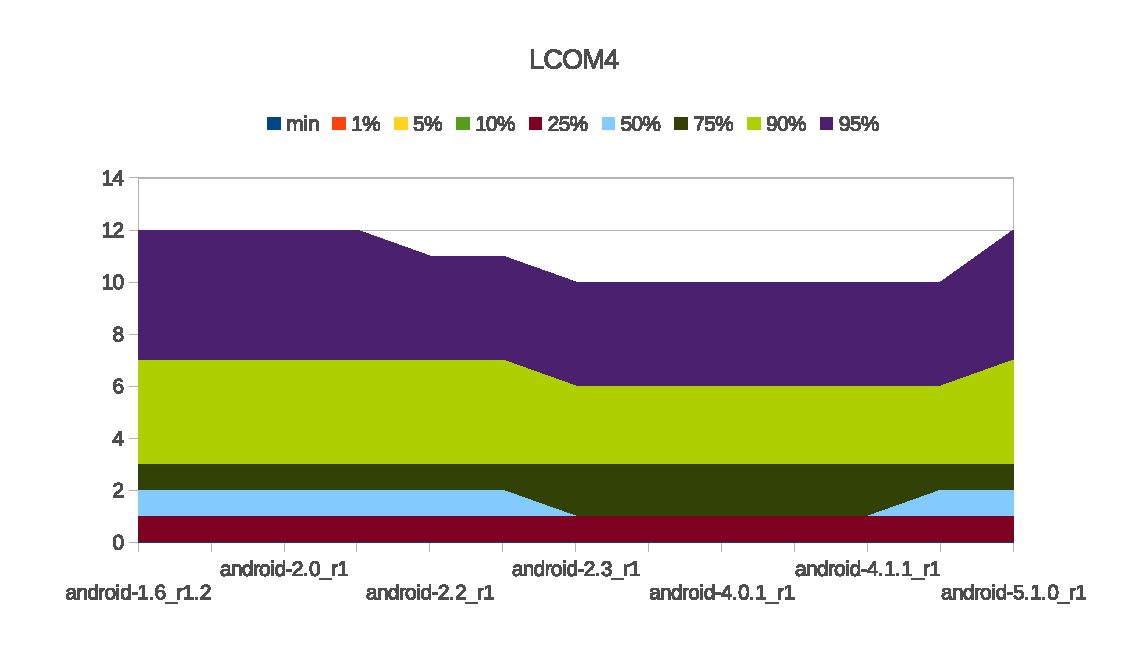
\includegraphics [keepaspectratio=true,scale=0.85]{figuras/graphs/lcom4_android.eps}
\caption{Evolução da métrica LCOM4 ao longo das versões da API}
\label{fig:lcom4_android}
\end{figure}

A Figura~\ref{fig:lcom4_android} apresenta a continuidade dos valores para LCOM na API do android, que, mesmo quado variam de uma versão para outra, retornam aos valores antigos, circulando acerca de um pequeno range de valores. Para o percentil 75, que representa valores muito frequentes, o gráfico demonstra uma linha reta horizontal em verde escuro que não desviou do valor 3 em nenhuma versão da API.

\begin{table}[!htb]
\centering
\scalefont{.7}
\documentclass[a4paper]{article}
\usepackage[T1]{fontenc}
\usepackage[latin1]{inputenc}
\begin{document}
\begin{tabular}{|l|l|l|l|l|l|l|l|l|l|l|l|}
\hline
version&min&1\%&5\%&10\%&25\%&50\%&75\%&90\%&95\%&99\%&max\\
\hline
android-1.6\_r1.2&0&0&0&0&1&2&3&7&12&33&254\\
\hline
android-1.6\_r1.5&0&0&0&0&1&2&3&7&12&33&254\\
\hline
android-2.0\_r1&0&0&0&0&1&2&3&7&12&32&253\\
\hline
android-2.1\_r2.1p2&0&0&0&0&1&2&3&7&12&33&253\\
\hline
android-2.2\_r1&0&0&0&0&1&2&3&7&11&31&253\\
\hline
android-2.2.3\_r2&0&0&0&0&1&2&3&7&11&31&253\\
\hline
android-2.3\_r1&0&0&0&0&1&1&3&6&10&31&253\\
\hline
android-2.3.7\_r1&0&0&0&0&1&1&3&6&10&31&253\\
\hline
android-4.0.1\_r1&0&0&0&0&1&1&3&6&10&32.9200000000001&253\\
\hline
android-4.0.4\_r2.1&0&0&0&0&1&1&3&6&10&32&253\\
\hline
\end{tabular}
\end{document}

\caption{\textit{Lack of Cohesion in Methods} no Android}
\label{tab:lcom4_android}
\end{table}

A Tabela~\ref{tab:lcom4_android} demonstra que em todas as versões da API Android o valor muito frequente é 3. De 3 a 7 são valores frequentes, e de 7 a 12 pouco frequentes. Valores acima de 12 não são frequentes no sistema. 

Embora o valor ideal de LCOM4 seja 1, valores maiores que 1 não são totalmente estranhos. Muitas classes são criadas para representar alguma entidade real, e para manter seu valor semântico devem desempenhar alguns papéis distintos ao mesmo tempo. E isso é mais frequentemente visto em projetos que contém muitos dispositivos físicos acessíveis e utilizáveis no sistema. 

Em dispositivos móveis, por exemplo, tarefas de tirar foto e capturar vídeo, que são bem distintas, são reunidas na classe câmera, que representa o dispositivo físico que contempla essas funcionalidades. Essa representação de hardware em uma classe específica auxilia a manter uma maior organização no código, e mesmo que sejam tarefas distintas, resultando possivelmente em um maior valor de LCOM4, as classes ainda podem ser consideradas coesas. Fazer a separação da representação de um dispositivo físico em diversas classes pode não ser tão fácil quanto em um projeto com objetos mais ``abstratos'', que podem ser mais facilmente separados sem prejudicar o entendimento da estrutura do sistema.

\begin{table}[!htb]
\centering
\scalefont{.7}
\begin{tabular}{|l|l|l|l|l|l|l|l|l|l|l|l|l|}
\hline
app&classes&min&1\%&5\%&10\%&25\%&50\%&75\%&90\%&95\%&99\%&max\\
\hline
Launcher2&161&0&0&1&1&1&2&4&7.1&10.1&22.23&42\\
\hline
Settings&722&0&0&0&0&1&1&3&5&6&10.8&44\\
\hline
Camera2&462&0&0&0&0&1&1&3&7&11&22&135\\
\hline
Bluetooth&239&0&0&0&1&1&2&3&8&10.15&21.52&27\\
\hline
QuickSearchBox&196&0&0&1&1&1&2&3&6&13&21.18&30\\
\hline
Calculator&10&1&1&1&1&1&1&2&5.6&6.8&7.76&8\\
\hline
SoundRecorder&6&1&1&1&1&1&2&2&2&2&2&2\\
\hline
Terminal&17&0&0.15&0.75&1&1&1&3&6.5&10.75&17.35&19\\
\hline
PackageInstaller&19&0&0.17&0.85&1&1&1&3&4.3&5.3&6.66&7\\
\hline
Dialer&215&0&0&0&1&1&2&3&6&9&15.87&28\\
\hline
Browser&259&0&0&1&1&1&2&4&6&9&32.87&54\\
\hline
InCallUI&117&0&0&0&0&1&2&4&6&8&14.95&25\\
\hline
LegacyCamera&214&0&0&0&0.2&1&2&3&6&7.4&22.52&47\\
\hline
Gallery2&895&0&0&0&0&1&2&3&6&9&17.07&38\\
\hline
BasicSmsReceiver&5&1&1&1&1&1&1&1.25&1.7&1.85&1.97&2\\
\hline
UnifiedEmail&872&0&0&0&1&1&2&3&6&10.5&25.6&76\\
\hline
Launcher3&354&0&0&0&0&1&2&4&7&11&33.84&51\\
\hline
Music&75&0&0&0&1&1&2&5&15.7&19.75&45.08&48\\
\hline
Camera&253&0&0&0&1&1&2&3&6&13&39.86&65\\
\hline
Email&400&0&0&0&1&1&2&3&7&13&46.02&144\\
\hline
Nfc&178&0&0&0&1&1&1&3&9.4&18&25.48&29\\
\hline
Gallery&89&0&0.87&1&1&1&1.5&3.25&6&9&17.52&21\\
\hline
ContactsCommon&292&0&0&0&1&1&2&3&6&7.5&17.1&77\\
\hline
Contacts&265&0&0&0&1&1&2&4&6&8&15.11&21\\
\hline
DeskClock&121&0&0&0&1&1&2&3&5&5.05&11.24&24\\
\hline
HTMLViewer&4&1&1&1&1&1&1&1.5&1.8&1.9&1.98&2\\
\hline
Calendar&216&0&0&0&1&1&2&3&5&6.3&31.32&51\\
\hline
Exchange&135&0&0&0&1&1&2&3&6&12&21.35&32\\
\hline
\end{tabular}

\caption{\textit{Lack of Cohesion in Methods} nos aplicativos nativos}
\label{tab:lcom4_apps}
\end{table}

\citeonline{meirelles2013} define para projetos Java intervalos de 0 a 3, 4 a 7, e 8 a 12 para os percentis 75, 90 e 95, respectivamente. Os resultados encontrados aqui acompanharam muito bem esses intervalos.

LCOM4 também contabiliza classes de modelo, e no caso do Java, os \textit{getters} e \textit{setters} acarretam no aumento do valor do resultado da métrica\cite{meirelles2013}, entretanto foi verificado, em alguns projetos utilizados como teste, que a ferramenta Analizo não contabilizou esses métodos. Como pode ser visto na Tabela~\ref{tab:lcom4_apps}, os intervalos 0 a 4, 4 a 7, e 7 a 12 são válidos para a grande maioria dos aplicativos. Os resultados são muito parecidos com os valores para a API, sendo que a métrica só aumenta em 1 no percentil 75.

\subsection{Afferent Connections per Class}

\begin{table}[!htb]
\centering
\scalefont{.7}
\begin{tabular}{|l|l|l|l|l|l|l|l|l|l|l|l|l|}
\hline
version&classes&min&1\%&5\%&10\%&25\%&50\%&75\%&90\%&95\%&99\%&max\\
\hline
android-1.6\_r1.2&5745&0&0&0&0&0&0&3&12&26&137&1820\\
\hline
android-1.6\_r1.5&5745&0&0&0&0&0&0&3&12&26&137&1820\\
\hline
android-2.0\_r1&6331&0&0&0&0&0&0&3&11&25&139&1953\\
\hline
android-2.1\_r2.1p2&6360&0&0&0&0&0&0&3&11&25&139.41&1970\\
\hline
android-2.2\_r1&7352&0&0&0&0&0&0&3&12&25.45&132.98&2027\\
\hline
android-2.2.3\_r2&7358&0&0&0&0&0&0&3&12&26&132.86&2028\\
\hline
android-2.3\_r1&8093&0&0&0&0&0&0&3&11&25&114.08&2052\\
\hline
android-2.3.7\_r1&8240&0&0&0&0&0&0&3&11&25&115.22&2070\\
\hline
android-4.0.1\_r1&11709&0&0&0&0&0&0&3&11&24&122&2681\\
\hline
android-4.0.4\_r2.1&11851&0&0&0&0&0&0&3&11&24&121.5&2711\\
\hline
android-4.1.1\_r1&14115&0&0&0&0&0&0&3&11&24&117.86&2965\\
\hline
android-4.3.1\_r1&15472&0&0&0&0&0&0&3&12&25&121&3789\\
\hline
android-5.1.0\_r1&20129&0&0&0&0&0&0&3&11&22&99.72&4180\\
\hline
\end{tabular}

\caption{\textit{Afferent Connections per Class} no Android}
\label{tab:acc_android}
\end{table}

\begin{figure}[!htb]
\centering
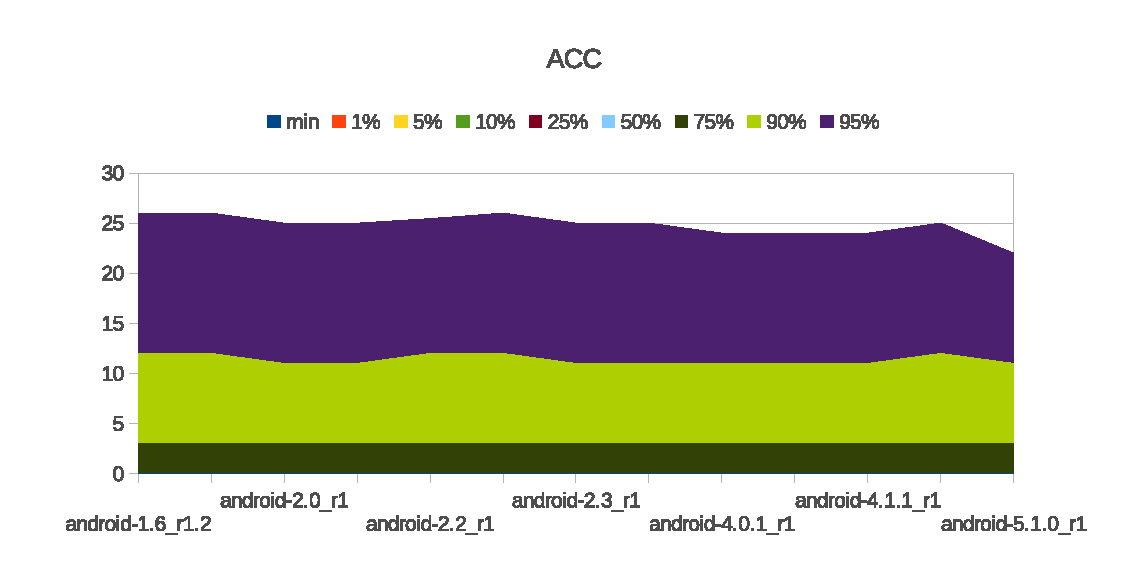
\includegraphics [keepaspectratio=true,scale=0.85]{figuras/graphs/acc_android.eps}
\caption{Evolução da métrica ACC ao longo das versões da API}
\label{fig:acc_android}
\end{figure}

A Figura~\ref{fig:acc_android} e a Tabela~\ref{tab:acc_android} demonstram que os valores da métrica ACC para os percentis 75, 90 e 95 não passam de 3, 12 e 26, respectivamente. \citeonline{oliveira2013} define os intervalos 0 a 2, 2 a 7, e 7 a 15 como excelente, bom e regular para os valores dessa métrica. \citeonline{meirelles2013} define como referência para Java os intervalos 0 a 1, 1 a 5, e 5 a 12 para os percentis 75, 90 e 95, respectivamente.

Os valores encontrados para o Android estão altos quando comparados com esses estudos, e portanto estes não são bem aplicáveis à API do Android, que, como podemos ver na Figura~\ref{fig:acc_android}, contém valores que não parecem ter tendência clara de reduzir para os intervalos considerados bons. A variância dentre as versões da API aqui analisadas é muito baixa, uma vez que quase os mesmos valores podem ser vistos ao longo das versões. Como os intervalos encontrados são constantes ao longo das versões, parecem refletir o design do sistema e podem ser utilizados como referência.

\begin{table}[!htb]
\centering
\scalefont{.7}
\begin{tabular}{|l|l|l|l|l|l|l|l|l|l|l|l|l|}
\hline
app&classes&min&1\%&5\%&10\%&25\%&50\%&75\%&90\%&95\%&99\%&max\\
\hline
Launcher2&161&0&0&0&0&0&2&5.25&17.1&26.1&92.38&110\\
\hline
Settings&722&0&0&0&0&0&0&2&6&10&26.6&307\\
\hline
Camera2&462&0&0&0&0&0&0&3&10&18&43.6&122\\
\hline
Bluetooth&239&0&0&0&0&0&1&5&16&31&81.5&169\\
\hline
QuickSearchBox&196&0&0&0&0&0&0&2&6&9&24.56&54\\
\hline
Calculator&10&0&0&0&0&0&2&2&2.4&3.2&3.84&4\\
\hline
Terminal&17&0&0&0&0&0&1&2.25&5&8.25&13.65&15\\
\hline
PackageInstaller&19&0&0&0&0&0&0.5&1&3.3&4.3&5.66&6\\
\hline
Dialer&215&0&0&0&0&0&1&3&6.7&11&16.87&35\\
\hline
Browser&259&0&0&0&0&0&1&3&8&15.15&58.16&122\\
\hline
InCallUI&117&0&0&0&0&0&1&3&6.5&10.5&25.55&93\\
\hline
LegacyCamera&214&0&0&0&0&0&2&6&11.8&16&53.4&91\\
\hline
Gallery2&895&0&0&0&0&0&1&4&11&21.35&75&150\\
\hline
BasicSmsReceiver&5&0&0&0&0&0&0&0.25&0.7&0.85&0.97&1\\
\hline
UnifiedEmail&872&0&0&0&0&0&0&3&10&16&53&160\\
\hline
Launcher3&354&0&0&0&0&0&1&4&14.8&21.8&72.24&124\\
\hline
Music&75&0&0&0&0&0&0&1&2&2.7&6.7&14\\
\hline
Camera&253&0&0&0&0&0&2&5&11.9&18.25&57.13&103\\
\hline
Email&400&0&0&0&0&0&0&1&6&18.1&40.22&201\\
\hline
Nfc&178&0&0&0&0&0&1&4&11.4&18&61.48&67\\
\hline
Gallery&89&0&0&0&0&0&1&4&8.3&13&49.13&50\\
\hline
ContactsCommon&292&0&0&0&0&0&0&1&7&15&69.4&108\\
\hline
Contacts&265&0&0&0&0&0&0&2&5&10&14.37&30\\
\hline
DeskClock&121&0&0&0&0&0&1&6&12&20&32.91&37\\
\hline
HTMLViewer&4&0&0&0&0&0&0&1&1.6&1.8&1.96&2\\
\hline
Calendar&216&0&0&0&0&0&0&4&9&18&29.44&45\\
\hline
Exchange&135&0&0&0&0&0&0&2&5&10.05&71.54&108\\
\hline
\end{tabular}

\caption{\textit{Afferent Connections per Class} nos aplicativos nativos}
\label{tab:acc_apps}
\end{table}

A Tabela~\ref{tab:acc_apps} demonstra que os valores para os aplicativos do sistema também são maiores que os intervalos definidos em outros estudos. Entretanto, eles são mais parecidos com os valores encontrados dentro da própria API, mais uma vez refletindo a semelhança de aplicativos em relação a mesma, e demonstrando um certo padrão para códigos relacionados ao Android. Para a grande maioria dos aplicativos, os percentis 75, 90 e 95 não ultrapassam os valores 4, 12 e 22, respectivamente.

Classes de modelo tendem a ser utilizadas como variável de instância em diversos lugares em um aplicativo, e portanto podem ter valores de ACC mais altos. Verificou-se que referências estáticas não são contabilizadas pela ferramenta Analizo para o cálculo de ACC. Em suma, no Analizo só aumenta o ACC em escopo de objeto, não de classe, ou seja, se a classe for utilizada como objeto em algum contexto, tendo alguma variável ou método acessado através desse objeto.

Consideramos então os seguintes intervalos para o Android:

\begin{itemize}
\item Para o percentil 75, ACC igual a 3 para a API e 4 para aplicativos;
\item 12 é um limite recorrente para o percentil 90 para aplicativos e para a API;
\item Para o percentil 95 em diante, aplicativos tem um valor médio menor que a API, estando com limites até 22 e 26, respectivamente.
\end{itemize}

\subsection{Coupling Factor}

\begin{table}[!htb]
\centering
\scalefont{.7}
\begin{tabular}{|l|l|l|}
\hline
version&classes&cof\\
\hline
android-1.6\_r1.2&5745&0.0013695147\\
\hline
android-1.6\_r1.5&5745&0.001369545\\
\hline
android-2.0\_r1&6331&0.0012379467\\
\hline
android-2.1\_r2.1p2&6360&0.0012384764\\
\hline
android-2.2\_r1&7352&0.0010625123\\
\hline
android-2.2.3\_r2&7358&0.0010616483\\
\hline
android-2.3\_r1&8093&0.0009540904\\
\hline
android-2.3.7\_r1&8240&0.000937113\\
\hline
android-4.0.1\_r1&11709&0.0007400012\\
\hline
android-4.0.4\_r2.1&11851&0.0007300137\\
\hline
android-4.1.1\_r1&14115&0.0005968253\\
\hline
android-4.3.1\_r1&15472&0.0005764279\\
\hline
&&\\
\hline
&&\\
\hline
&&\\
\hline
&&\\
\hline
&&\\
\hline
&&\\
\hline
&&\\
\hline
&&\\
\hline
&&\\
\hline
&&\\
\hline
&&\\
\hline
&&\\
\hline
&&\\
\hline
&&\\
\hline
&&\\
\hline
\end{tabular}

\caption{\textit{Coupling Factor} no Android}
\label{tab:cof_android}
\end{table}

\begin{figure}[!htb]
\centering
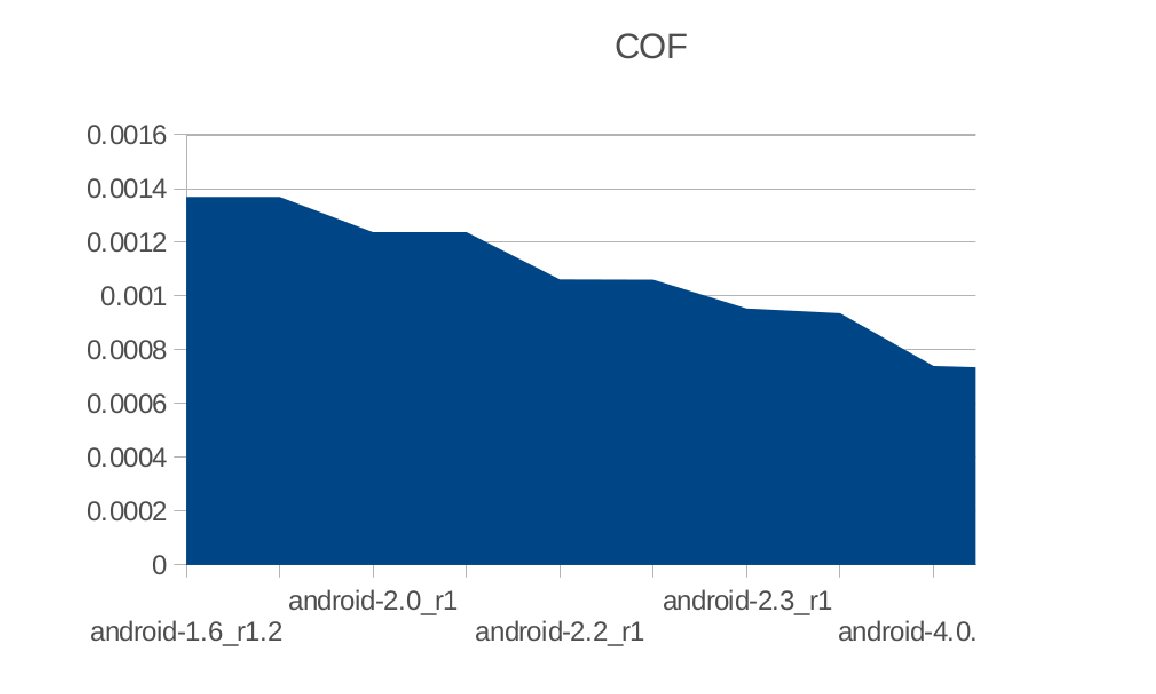
\includegraphics [keepaspectratio=true,scale=0.7]{figuras/graphs/cof_android.eps}
\caption{Evolução da métrica COF ao longo das versões da API}
\label{fig:cof_android}
\end{figure}

%TODO atualizar valores quando obtiver mais versões

O valor de COF para a API do Android ao longo de suas versões caiu de 0.13\% para 0.057\%, como pode ser visto na Figura~\ref{fig:cof_android} e na Tabela~\ref{tab:cof_android}. Isso se dá pelo fato de que, como demonstrado na seção anterior, o valor de ACC permanece relativamente constante enquanto o número de classes aumenta significativamente a cada versão. Essencialmente, o sistema se mostra cada vez mais desacoplado e consequentemente manutenível. 

\begin{table}[!htb]
\centering
\scalefont{.7}
\begin{tabular}{|l|l|l|}
\hline
app&classes&total\_cof\\
\hline
HTMLViewer&4&0.3333333333\\
\hline
BasicSmsReceiver&5&0.0833333333\\
\hline
Calculator&10&0.1666666667\\
\hline
Terminal&17&0.1416666667\\
\hline
PackageInstaller&19&0.0653594771\\
\hline
Music&75&0.0111069974\\
\hline
Gallery&89&0.0432340648\\
\hline
InCallUI&117&0.028035982\\
\hline
DeskClock&121&0.0343837535\\
\hline
Exchange&135&0.0253619122\\
\hline
Launcher2&161&0.0415487421\\
\hline
Nfc&178&0.0273497689\\
\hline
QuickSearchBox&196&0.0111551679\\
\hline
LegacyCamera&214&0.0230312694\\
\hline
Dialer&215&0.0119125971\\
\hline
Calendar&216&0.014844599\\
\hline
Bluetooth&239&0.0259014998\\
\hline
Camera&253&0.0195566939\\
\hline
Browser&259&0.0161825476\\
\hline
Contacts&265&0.0070284595\\
\hline
ContactsCommon&292&0.0110795118\\
\hline
Launcher3&354&0.0148564254\\
\hline
Email&400&0.0083122379\\
\hline
Camera2&462&0.0079222861\\
\hline
Settings&722&0.0040414548\\
\hline
UnifiedEmail&872&0.0044023912\\
\hline
Gallery2&895&0.0055753048\\
\hline
\end{tabular}

\caption{\textit{Coupling Factor} nos aplicativos nativos}
\label{tab:cof_apps}
\end{table}

A Tabela~\ref{tab:cof_apps} apresenta os valores para os aplicativos e nela é possível perceber que o valor de COF não é sempre inversamente proporcional a quantidade de classes como já comentado, embora ele realmente tenha a tendencia a diminuir com o aumento do número de classes. Para os aplicativos, tivemos um range de 33\% para o menor dos projetos, com apenas 4 classes, e 0.4\% para um dos maiores aplicativos.

\citeonline{ferreira2009} apresenta como intervalos os valores de 0 a 0.02 (2\%) como bons , 0.02 a 0.14 (14\%) como regulares, e 0,14 em diante como valores ruins. Podemos perceber que os valores para o sistema Android estão bem abaixo desses valores, sendo considerados então excelentes valores para o fator de acoplamento. Já os aplicativos demonstraram que se mantém nos valores bons quando passam a ter por volta de 200 classes, mas quado muito pequenos se mostraram em sua maioria regulares nessa escala. 

Os intervalos aqui não são considerados em função de seus percentis, mas as seguintes observações podem ser feitas:

\begin{itemize}
\item Espera-se que o valor de COF para o sistema se mostre cada vez menor à medida que novas versões surgem;
\item Aplicativos desenvolvidos para o Android, quando muito pequenos, até poucas dezenas de classes, tendem a ficar abaixo de 10\%, e não devem ultrapassar os 14\% no valor de COF. Valores bem menores ainda podem ser obtidos e são preferíveis;
\item A medida que ganham tamanho de várias dezenas à poucas centenas de classes, os valores de COF para aplicativos não devem ultrapassar os 4\%, entretanto é recomendável que fique abaixo de 2\%. Quando chegam a várias centenas de classes, os valores devem ser menores que 1\%.
\end{itemize}

\subsection{Observações acerca das métricas}

\begin{table}[!htb]
\centering
\scalefont{.8}
\begin{tabular}{|l|l|l|}
\hline
Métrica & Intervalos                                                                                          & Rótulo                                                                                                                      \\ \hline
AMLOC   & \begin{tabular}[c]{@{}l@{}}{[}0, 14{]}\\ {[}14, 31{]}\\ {[}31, 55{]}\\ {[}55, ...{]}\end{tabular}   & \begin{tabular}[c]{@{}l@{}}Muito Frequente\\ Frequente\\ Pouco Frequente\\ Não Frequente\end{tabular}                       \\ \hline
ACCM    & \begin{tabular}[c]{@{}l@{}}{[}0, 2{]}\\ {[}2, 4{]}\\ {[}4, 6{]}\\ {[}6, ...{]}\end{tabular}         & \begin{tabular}[c]{@{}l@{}}Muito Frequente\\ Frequente\\ Pouco Frequente\\ Não Frequente\end{tabular}                       \\ \hline
RFC     & \begin{tabular}[c]{@{}l@{}}{[}0, 31{]}\\ {[}31, 85{]}\\ {[}85, 140{]}\\ {[}140, ...{]}\end{tabular} & \begin{tabular}[c]{@{}l@{}}Muito Frequente\\ Frequente\\ Pouco Frequente\\ Não Frequente\end{tabular}                       \\ \hline
DIT     & \begin{tabular}[c]{@{}l@{}}{[}0, 1{]}\\ {[}1, 2{]}\\ {[}2, 4{]}\\ {[}4, ...{]}\end{tabular}         & \begin{tabular}[c]{@{}l@{}}Muito Frequente\\ Frequente\\ Pouco Frequente\\ Não Frequente\end{tabular}                       \\ \hline
NOC     & \begin{tabular}[c]{@{}l@{}}0\\ 1\\ 2\\ {[}3, ...{]}\end{tabular}                                    & \begin{tabular}[c]{@{}l@{}}Muito Frequente\\ Frequente\\ Pouco Frequente\\ Não Frequente\end{tabular}                       \\ \hline
LCOM4   & \begin{tabular}[c]{@{}l@{}}{[}0, 3{]}\\ {[}3, 7{]}\\ {[}7, 12{]}\\ {[}12, ...{]}\end{tabular}       & \begin{tabular}[c]{@{}l@{}}Muito Frequente\\ Frequente\\ Pouco Frequente\\ Não Frequente\end{tabular}                       \\ \hline
ACC     & \begin{tabular}[c]{@{}l@{}}{[}0, 3{]}\\ {[}3, 12{]}\\ {[}12, 26{]}\\ {[}26, ...{]}\end{tabular}     & \begin{tabular}[c]{@{}l@{}}Muito Frequente\\ Frequente\\ Pouco Frequente\\ Não Frequente\end{tabular}                       \\ \hline
COF     & \begin{tabular}[c]{@{}l@{}}até 14\%\\ até 4\%\\ até 2\%\end{tabular}                                & \begin{tabular}[c]{@{}l@{}}Para poucas dezenas de classes\\ Para poucas centenas de classes\\ Para várias centenas de classes\end{tabular} \\ \hline
\end{tabular}
\caption{Intervalos definidos para sistema Android}
\label{tab:final_table_android}
\end{table}

A Tabela~\ref{tab:final_table_android} apresenta um resumo dos intervalos definidos para a API do sistema Android ao longo dessa seção. Embora algumas métricas tenham um indicativo de um problema pontual, como explicado no Capítulo~\ref{cap:referencial_teorico} e em outras seções deste capítulo, nenhuma das métricas discutidas neste trabalho deve ser analisada isoladamente.

Valores baixos de AMLOC são sempre preferíveis, pois métodos mais enxutos tem menor responsabilidade, portanto estão mais sujeitos a reuso, e também são mais fáceis de se ler e se modificar. Entretanto essa métrica é preciso ser analisada em conjunto com outras métricas, como LCOM4 e RFC. Uma classe com muitos métodos privados pequenos tende a ter um valor maior de RFC, o que não implica que esteja mal projetada, desde que os métodos ali presentes estejam bem posicionados segundo o padrão de projeto OO especialista da informação, mantendo por consequência um baixo valor de LCOM4. Como referência geral de resultados para AMLOC, quanto menor o valor, melhor o resultado.

O resultados para a métrica ACCM, que é uma métrica bastante difundida e tem sua aplicabilidade bem clara, relacionados aos AMLOC, dão subsídio para reafirmar que os valores da métrica AMLOC devem ser os menores possíveis para uma boa arquitetura orientada a objetos.

Entender a relação entre ACCM e AMLOC é importante também para pensar em possibilidade de refatoração de um código fonte alvo. Estão claras as consequências de se ter uma alta complexidade ciclomática, mas essa discussão nos leva rapidamente a ter a ideia de verificar os métodos da classe e avaliar se seu comportamento está tão enxuto como deveria ser, se algum método não está fazendo mais do que propõe. As vezes dividir o comportamento em tarefas menores possa ser uma solução viável. Dividir o comportamento de um método em 2 provavelmente vai acarretar no aumento da métrica RFC, mas mais uma vez ressalto que o valor de RFC não deve ser analisado por si só. É importante ficar de olho também em métricas como a LCOM quando fazendo esse tipo de refatoração, pois as vezes uma tarefa menor que foi extraída de um método não está coesa na classe onde está e muitas vezes até já esteja implementada em uma outra classe que tem responsabilidade mais congruente com essa tarefa. Remover esse tipo de código duplicado ajuda a reduzir a falta de coesão dentro de uma classe, e todas essas melhorias derivaram do simples fato de perceber uma alta complexidade ciclomática em uma classe.

O ideal em uma classe é obter métodos pequenos com tarefas atômicas e bem definidas, que correspondam às responsabilidades dessa classe. A métrica RFC está diretamente relacionada a Number Of Methods (NOM), uma vez que um aumento neste ultimo implica necessariamente em um aumento em RFC. Uma classe que tenha alto RFC e muitos métodos (valor alto de NOM) pode indicar que está fazendo mais tarefas do que é sua responsabilidade fazer, necessitando talvez rever a sua implementação para aumentar sua coesão. Da mesma forma, um valor alto de RFC e valor baixo de NOM indica que uma classe está fazendo muito o uso de métodos de terceiros, podendo-se inferir que alguns métodos possam ser extraídos para essas classes que estão sendo tanto chamadas, com o objetivo de diminuir o acoplamento entre essas classes.

Alto valor de profundidade de árvore de herança em uma classe pode auxiliar no aumento da métrica RFC, uma vez que todos os comportamentos são herdados. Entretanto não é uma correlação direta significativa entre as duas, visto que a profundidade de herança raramente é alta para o sistema Android, como será discutido nas seções seguintes. Embora valor alto de DIT possa significar maior valor de RFC, valores muito altos de RFC tendem a indicar mais a falta de coesão e alto acoplamento, aumentando assim a complexidade estrutural da classe, e não uma profundidade de herança preocupante.

LCOM4 juntamente com RFC são bons indicadores da organização interna de uma classe, pois ambas as métricas dão subsídios para avaliar coesão. Essencialmente, métricas de coesão e acoplamento estão sempre relacionadas e são as métricas mais indicadas para avaliar a complexidade estrutural de uma classe. A ferramenta Analizo, por exemplo, calcula a métrica Structural Complexity (SC) como produto entre LCOM4 e CBO.

%As Tabelas~\ref{tab:cbo_android} e~\ref{tab:cbo_apps} demonstram que os valores encontrados para CBO na API e nos aplicativos são absurdamente grandes. Não foi encontrado um motivo para tal, podendo então haver algum tipo de problema na ferramenta de captura. O estudo conduzido por \citeonline{meirelles2013} utiliza a mesma ferramenta e não chegou a esses valores aqui encontrados em nenhum projeto, nem mesmo na análise do código fonte completo do sistema Android. Por não conseguirmos identificar exatamente o motivo dessa discrepância de valores, serão consideradas as métricas ACC e COF para acoplamento.

Dentro do escopo de um projeto, pela própria definição da métrica, o valor limite para ACC é o próprio número de classes. Embora o valor seja limitado pelo número de classes, não é possível perceber uma relação direta entre o crescimento do número de classes e o valor de ACC, sendo que essa métrica é mais relacionada à forma como o sistema foi pensado e desenhado do que com o seu tamanho. Entretanto, para análise longitudinal em um mesmo projeto, a relação entre número de classes e COF se mostra válida.

\section{Validação dos intervalos de referência}

Após a obtenção e analise de distribuição dos dados de métricas OO nas diferentes versões do Android e em aplicativos nativos, foram feitos alguns estudos para validar os intervalos de referência definidos na primeira seção deste capítulo. Também tinham o propósito de utilizar os dados obtidos para auxiliar desenvolvedores a não necessitarem de uma análise manual, assim como na proposta de comparação de aplicativos com a API.

Pensamos na criação um modelo de regressão que conseguisse predizer o valor ideal de uma métrica OO a partir de uma variável independente de tamanho que representasse a escala do projeto, de forma a obter um valor proporcional daquela métrica. O desenvolvedor então poderia comparar esse valor com o valor real da métrica que o código apresenta, e com os intervalos que foram definidos neste trabalho, e então verificar se mudanças estruturais devem ser feitas.

Um modelo de regressão iria aprender os valores ideais para API com os próprios dados crus das métricas, e então sera possível comparar esses resultados com os valores definidos manualmente através dos percentis, discutidos na primeira seção deste capítulo.

%Após identificadas as limitações e problemáticas com essa abordagem de regressão, o trabalho seguiu um novo caminho em direção à uma comparação mais direta. A ideia vem da proposição de que, julgando a API como um bom exemplo de código, valores próximos aos da API podem ser considerados bons por consequência. 

%O passo seguinte foi então avaliar a qualidade um aplicativo a partir da distancia da API no que diz respeito a métricas estáticas de código.

\subsection{Validação por regressão}

A seguir métricas base que foram inicialmente idealizadas para relativização das métricas por regressão polinomial:

\begin{enumerate}
\item Número de classes, realizando uma regressão em escopo de software.
\item Número de classes por pacote, resultando em uma regressão em escopo de ``módulo''.
\item NOM, realizando uma regressão em escopo de classe.
\item AMLOC, realizando uma regressão em escopo de classe.
\end{enumerate}

Não é possível idealizar esse resultado para métricas OO, mensuradas para cada classe, para entradas mais granularizadas como valores de métodos. A grande maioria das métricas tem seus valores para a classe como um todo, não podendo fazer distinção sobre a participação de cada método individualmente dentro daquele valor.

Nenhuma das formas propostas foi realmente implementada, apenas foi realizado uma discussão das possibilidades com as métricas que estavam disponíveis. Métricas de tamanho foram o alvo da regressão como variáveis independentes porque seriam uma forma de abstrair os resultados para projetos de diferentes escalas. Essencialmente os intervalos de valores anteriormente definidos seriam validados se a métrica estivesse de acordo com os mesmos para os parâmetros específicos do projeto sendo analisado, fazendo uma comparação entre o modelo de regressão e a análise manual subjetiva deste trabalho.

\subsubsection{Regressão em escopo de software}

A primeira observação que se faz sobre a realização de regressão em escopo de software utilizando os valores da evolução da API do sistema Android é capacidade de generalização de um modelo. De forma geral, o modelo seria criado com pontos com valores de número de classes variando de 5000 a 20000 classes. Como consequência, argumentamos que o modelo de regressão não teria uma boa capacidade de generalização para projetos muito pequenos, como acontece com aplicativos, que possuem muitas vezes apenas algumas dezenas de classes, e são o alvo principal para utilização dessa regressão. Da mesma forma, a capacidade de predição para projetos que contenham bem mais que 20000 classes também seria prejudicada, uma vez que o modelo de regressão não veria nenhum nesse intervalo. 

\begin{figure}[!htb]
\centering
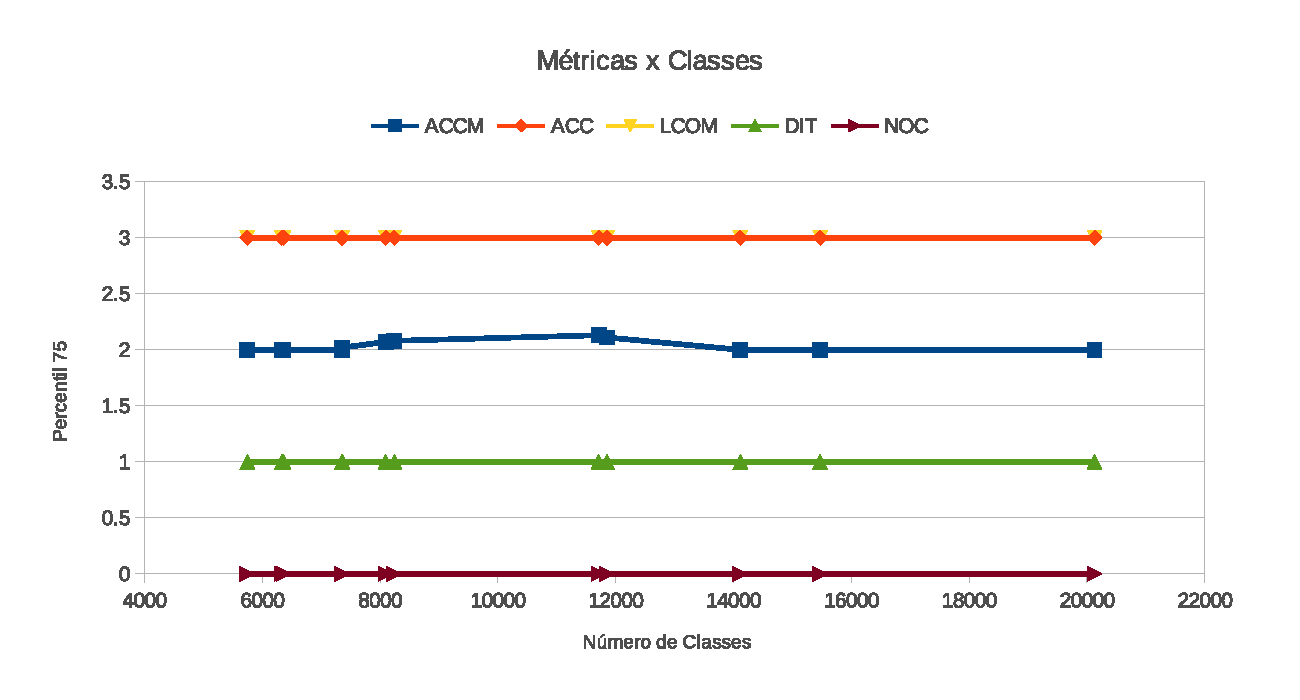
\includegraphics [keepaspectratio=true,scale=0.7]{figuras/metricasxclasses.eps}
\caption{Percentil 75 das métricas DIT, NOC, LCOM, ACC e ACCM}
\label{fig:metricasxclasses}
\end{figure}

\begin{figure}[!htb]
\centering
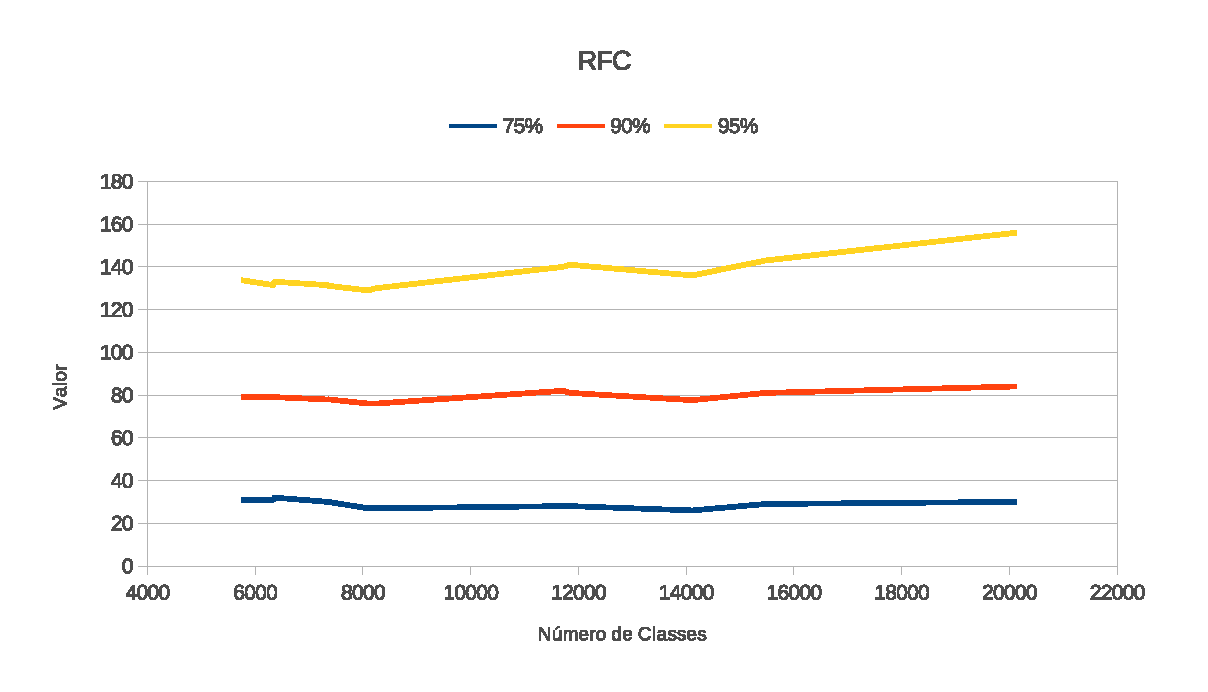
\includegraphics [keepaspectratio=true,scale=0.7]{figuras/rfcxclasses.eps}
\caption{Percentil 75, 90 e 95 de RFC em função do número de classes}
\label{fig:rfcxclasses}
\end{figure}

Para que isso pudesse ser realmente feito, os dados das métricas OO devem ser relacionados com as métricas de tamanho, demonstrando seu valor como dependente do valor dessas métricas. Se os dados obedecem um certo padrão, um funcional pode ser traçado para representar o comportamento dos mesmos. 

Como podemos ver na Figura~\ref{fig:metricasxclasses}, onde é traçado o percentil 75 em função do número de classes, as métricas DIT, NOC, ACC, LCOM4 e ACCM podem ser representadas por uma linha reta horizontal, enquanto RFC, plotada na Figura~\ref{fig:rfcxclasses}, tem dados mais dispersos mas ainda podem ser representados por uma reta horizontal sem perda significativa nos percentis 75 e 90, que correspondem a grande maioria dos dados. Nas tabelas e gráficos apresentados nas seção anterior pode ser confirmado que dentro de cada percentil de cada métrica a variação é pequena. Não foram plotados os valores de outros percentis aqui por diferenciação de escala que exigiria uma quantidade absurda de gráficos, além de não terem tanta importância quanto os valores muito frequêntes apresentados no percentil 75.

Para algumas métricas essa regressão parece ser possível, isto é, um funcional realmente pode ser traçado que representa a variação dos valores das métricas com o número de classes do projeto. Entretanto, para a ínfima variação nos percentis mais significativos para métricas importantes como ACC, LCOM4, DIT, NOC, RFC, ACCM, que são as principais métricas aqui analisadas, argumentamos que um valor referência se mostra tão útil quanto essa regressão, tornando-a desnecessária.

Além de poder utilizar um valor referência sem perda de valor semântico sobre o valor ideal da métrica, uma regressão em escopo de software da forma como foi proposta, pelo número de classes, não contém, com os dados aqui obtidos, um conjunto suficiente de dados para uma boa regressão. Em suma, temos poucas amostras para realizar esse estudo.

Como um pequeno problema adicional, os dados das métricas para os aplicativos se mostraram levemente diferentes para os dados da API do sistema, mesmo estando bem semelhantes, então argumentamos que utilizar apenas a API do sistema como insumo para o modelo de regressão resultaria em um modelo que não funciona tão bem para predizer valores de métricas de aplicativos. Para os aplicativos, que são projetos distintos, as métricas são extremamente dispersas em relação ao número de classes, tornando difícil representar bem os dados por um polinômio para realizar a regressão. 

Para realização de um modelo de regressão polinomial a nível de software, não foi encontrada ao longo deste trabalho, dadas restrições de tempo e escopo, outra métrica que representasse bem o tamanho do projeto para relativização do resultado das métricas OO. 

\subsubsection{Regressão em escopo de classe}

Como uma segunda tentativa na direção de uma regressão polinomial, foi verificada a possibilidade de utilizar valores das métricas para cada classe, e não para o projeto. Tentamos então avaliar o valor ideal de uma métrica para uma classe, dado alguma variável independente que represente de alguma forma seu tamanho.

\begin{figure}[!htb]
\centering
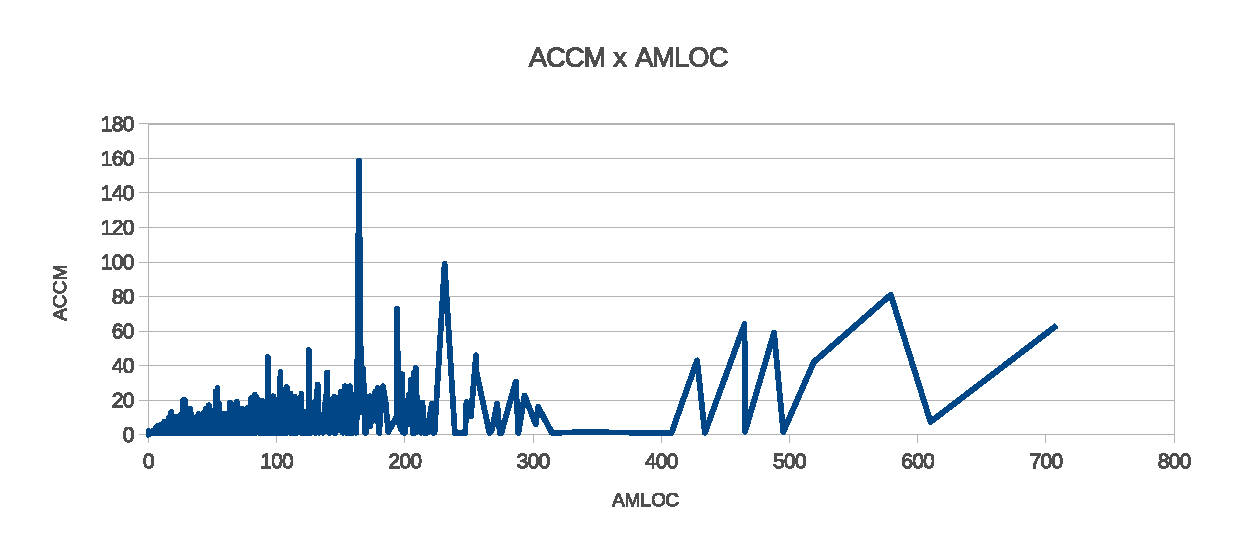
\includegraphics [keepaspectratio=true,scale=0.7]{figuras/accmxamloc510.eps}
\caption{ACCM em função de AMLOC na API versão 5.1.0}
\label{fig:accmxamloc510}
\end{figure}

\begin{figure}[!htb]
\centering
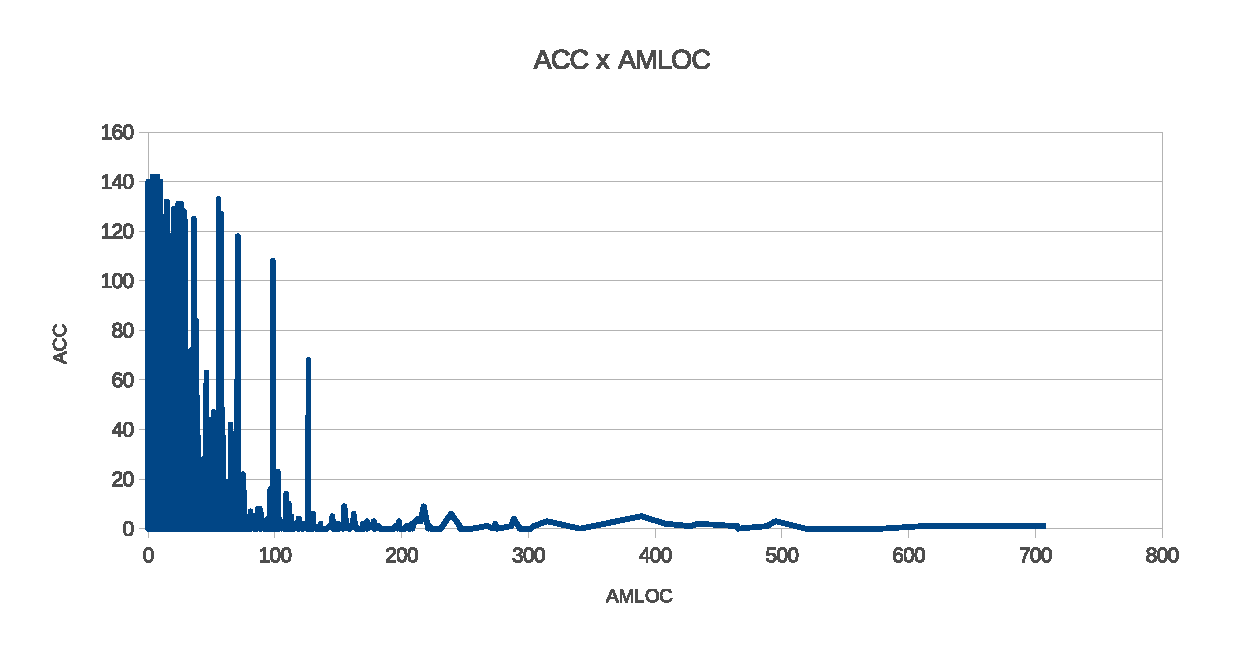
\includegraphics [keepaspectratio=true,scale=0.7]{figuras/accxamloc510.eps}
\caption{ACC em função de AMLOC na API versão 5.1.0}
\label{fig:accxamloc510}
\end{figure}


\begin{figure}[!htb]
\centering
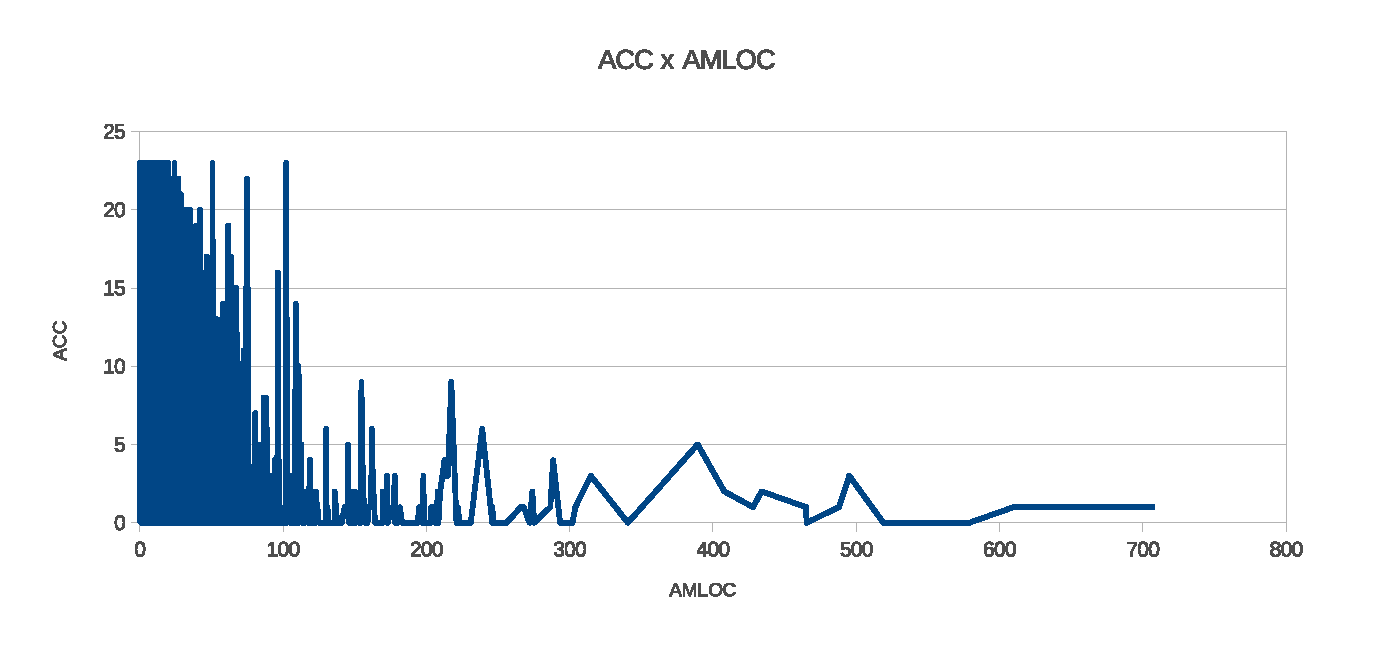
\includegraphics [keepaspectratio=true,scale=0.7]{figuras/accxamloc51095.eps}
\caption{ACC em função de AMLOC na API versão 5.1.0 com 95\% dos dados}
\label{fig:accxamloc51095}
\end{figure}

\begin{figure}[!htb]
\centering
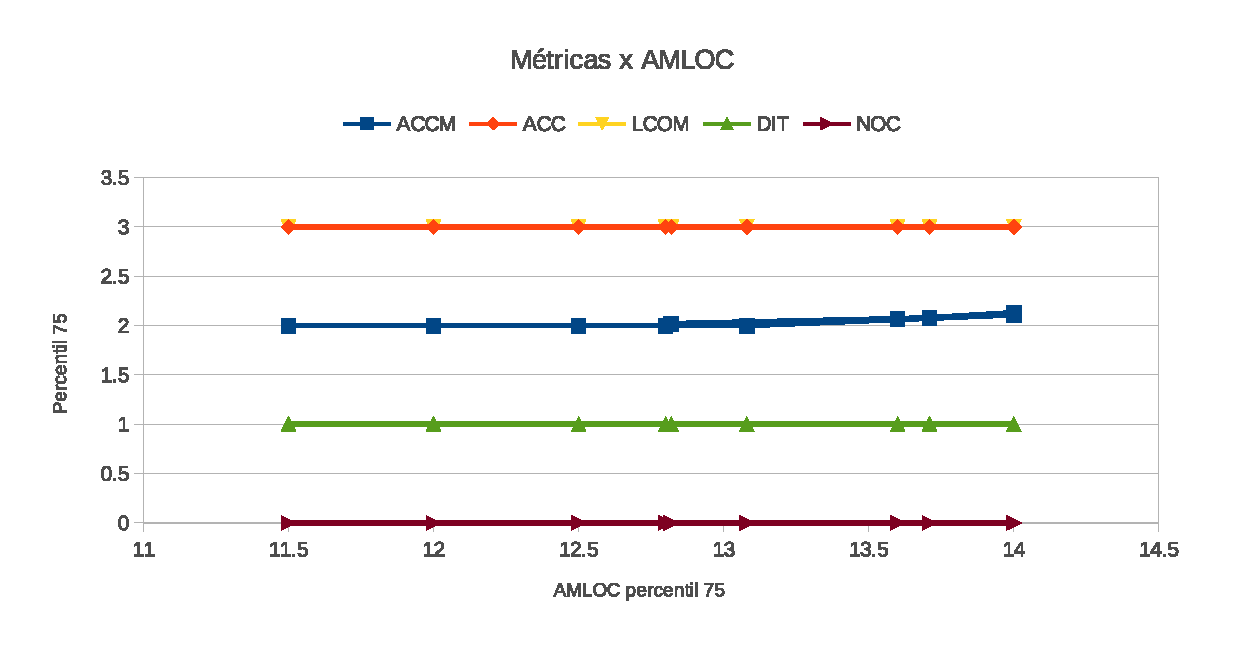
\includegraphics [keepaspectratio=true,scale=0.7]{figuras/metricasxamloc.eps}
\caption{DIT, NOC, LCOM, ACC e ACCM em função de AMLOC}
\label{fig:metricasxamloc}
\end{figure}

\begin{figure}[!htb]
\centering
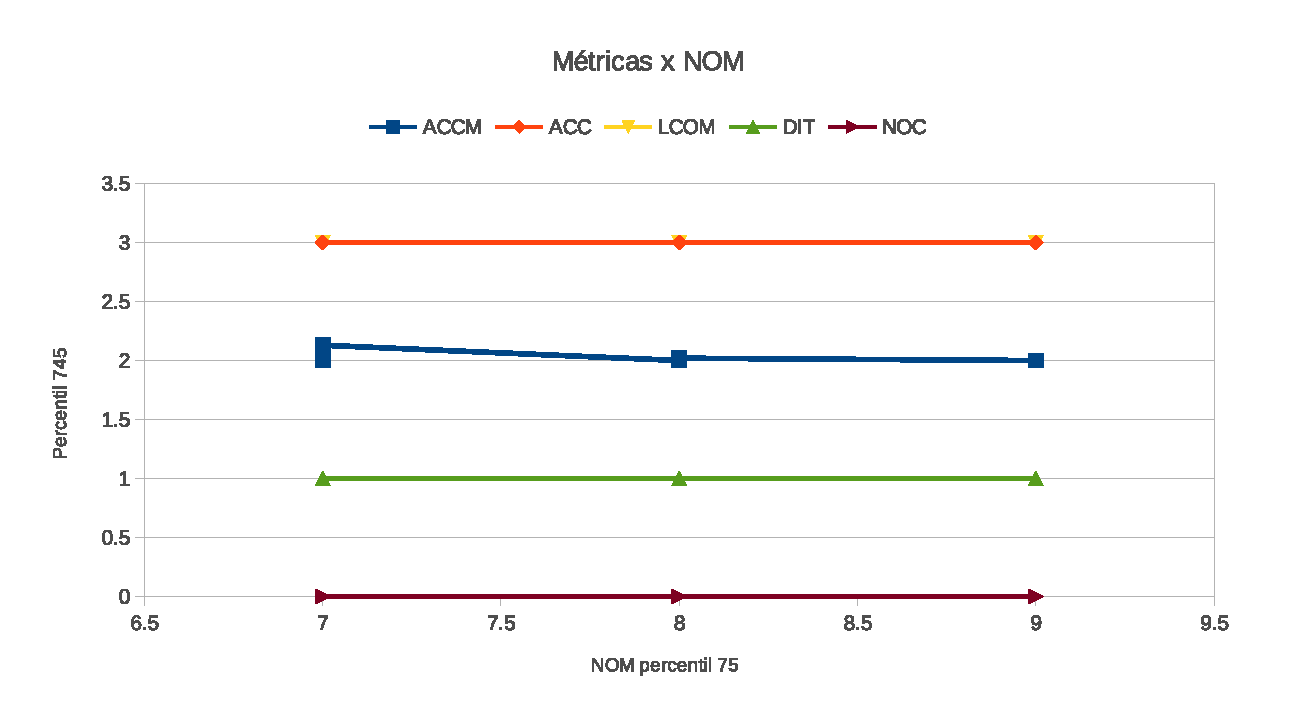
\includegraphics [keepaspectratio=true,scale=0.7]{figuras/metricasxnom.eps}
\caption{DIT, NOC, LCOM, ACC e ACCM em função de NOM}
\label{fig:metricasxnom}
\end{figure}

Cada classe dentro de cada versão seria uma amostra para esse método, que teria então um total de mais de 100000 classes. Pensando dessa forma o problema de escala do escopo de software seria resolvido.

O problema nessa abordagem é que as métricas de tamanho que podem ser utilizadas também se mostraram independentes dos valores das métricas OO. Como pode ser visto nas Figuras~\ref{fig:accmxamloc510} e~\ref{fig:accxamloc510}, os valores de ACC e ACCM parecem oscilar bastante. É importante notar que a parte de maior valor do gráfico representa uma quantidade muito pequena de amostras como os próprios percentis já descrevem. A Figura~\ref{fig:accxamloc51095} demonstra isso com o fato de que pouco menos de 5\% dos dados de maior valor foram retirados (1000 amostras), deixando aproximadamente os dados até o percentil 95, e a escala do gráfico caiu drasticamente. De forma geral, esses pontos de maior valor tem representação estatística muito pequena. Como os percentis representam a grande maioria de valores, iremos utilizá-los para fazer essa comparação, em vez do valor de cada classe.

Como mostram as Figuras~\ref{fig:metricasxamloc} e~\ref{fig:metricasxnom}, a variação das métricas OO em seus percentis mais representativos em função de AMLOC ou NOM é mínima e os dados se apresentam na forma de uma linha horizontal. Apenas ACCM tem uma suave relação crescente com AMLOC como já discutido na seção anterior. Na verdade, apenas pelo fato de essas métricas não variarem muito ao longo das versões, já se pode prever esse resultado.

\subsubsection{Regressão em escopo de pacote}

\begin{figure}[!htb]
\centering
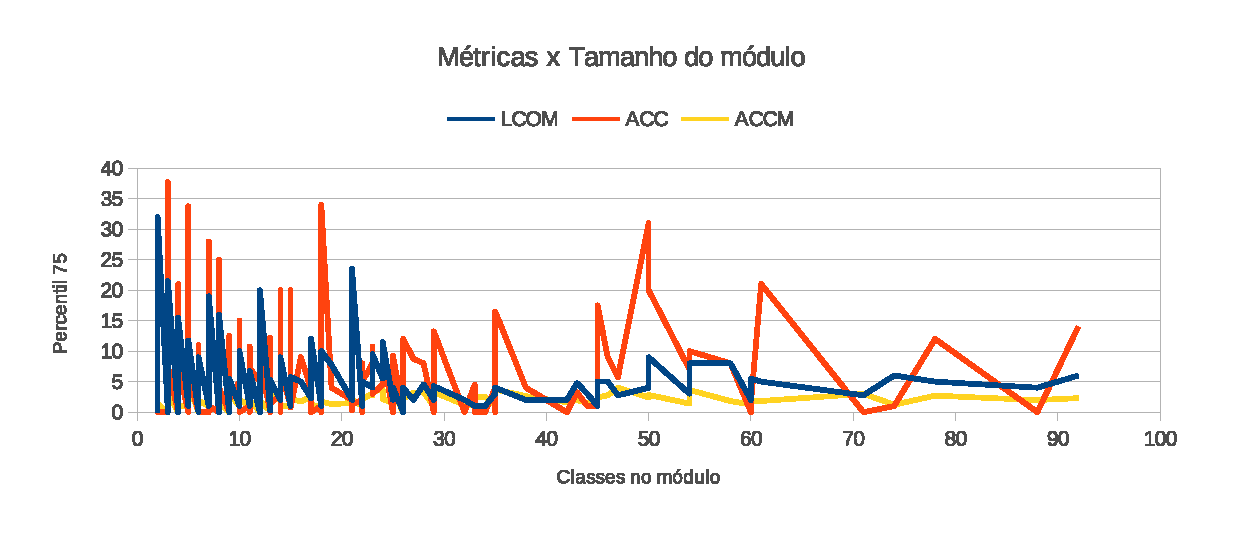
\includegraphics [keepaspectratio=true,scale=0.7]{figuras/metricasxtamanhomodulo.eps}
\caption{LCOM, ACC e ACCM em função do tamanho de módulo}
\label{fig:metricasxtamanhomodulo}
\end{figure}

Para fazer esse teste, foi separado cada pacote presente em cada versão do sistema, e utilizado como métrica de tamanho o número de classes nesse pacote. Os percentis para cada métrica eram calculados individualmente por pacote.

O problema encontrado nessa abordagem foi que as métricas eram dependentes do próprio pacote analisado e seu propósito, mas independentes de seu tamanho. Isso quer dizer que vários pacotes com mesmo número de classes apresentavam valores com nenhuma relação entre si. Basicamente, o mesmo problema de independência dos dados em relação a variável de tamanho foi encontrado aqui.

O gráfico da Figura~\ref{fig:metricasxtamanhomodulo} demonstra as métricas LCOM, ACC e ACCM para cada pacote em função dos seu número de classes. Podemos perceber que os valores tem uma grande variação que aparentemente independe do número de classes do pacote. Pacotes maiores podem parecer variar um pouco menos, mas isso se da pela quantidade menor de amostras em relação a pacotes pequenos.

Emfim, regressão neste contexto de métricas OO e métricas de tamanho não se mostrou um esforço válido para auxiliar desenvolvimento futuro de aplicativos. Mesmo no caso do escopo de software onde os dados podiam ser representados por um funcional, como a maioria dos valores se mostrou quase invariável ao longo das versões, ou com intervalos fixos, utilizar intervalos de referência tem tanta utilidade quanto uma regressão apresentaria. 

\section{Comparação de similaridade com a API}

Como foi comentado na seção anterior, as métricas OO não são dependentes de métricas de tamanho. Não foi encontrado uma forma de fazer a predição de um valor ideal de métrica para um determinado projeto sendo analisado.  

Entretanto, podemos abstrair um pouco os significados das métricas e avaliar o projeto como um todo fazendo uma comparação com o sistema. Valores para as métricas semelhantes aos do sistema podem ser considerados bons. Então, verificar o valor das métricas de forma relativa ao sistema ajuda a perceber se o valor está bom ou ruim sem necessariamente conhecer quais os valores bons ou ruins nesse contexto de desenvolvimento de aplicativos Android. 

Utilizando os valores identificados no início desse capítulo, neste trabalho considerados bons para o contexto Android, propomos então um cálculo de aproximação de aplicativos à API em termos de métricas estáticas de código. Essa comparação não se da de forma direta com o valor de uma classe de um projeto, mas sim para o projeto como um todo. Para isso, assim como na primeira seção, utilizamos os percentis 75, 90 e 95 dos valores de cada métrica dentro do projeto, com o objetivo de levar em conta a distribuição de valores da métrica dentro do sistema, visto que a média e a mediana não são sempre representativas para as métricas utilizadas \cite{meirelles2013}. A proposta de cálculo de similaridade da API então verifica as diferenças entre cada percentil do app e cada percentil da API, normalizados, e então unifica as diferenças entre as métricas em um só valor. 

\subsection{Normalização de valores}

Como as métricas geralmente se mostraram independentes, uma comparação direta pode ser bastante útil. Entretanto, obter um valor apenas de similaridade para a API não é efetivo se as métricas tem diferentes grandezas de valores. Consequentemente temos que fazer um trabalho de normalização dos valores das métricas para deixar todas as métricas com um mesmo \textit{range}, ou com grandezas equivalentes, e portanto ter uma certa equivalência, para calcular a distancia do app numa ideia semelhante ao que é feito com uma distancia euclidiana, onde todas as variáveis tem sua distancia unificada em um valor.

Normalizar métricas com valores sem um range específico pode ser bastante problemático. A métrica AMLOC, por exemplo, nada mais é do que a média de valores absolutos de tamanhos de métodos, que podem ser tão grandes quanto se queira. Dessa forma, não há um valor limite superior para os valores, embora o valor mínimo seja 0 pela própria forma de cálculo da métrica. Isso é válido para quase todas as métricas, com exceção de COF, que varia entre 0 e 1. Entretanto COF não tem uma abordagem de distribuição de valores por ser um valor único para o projeto, além do que é derivada de ACC, então não será utilizada no cálculo de distancia.

Para resolver este problema, foi considerado o fato de que termos um número grande de amostras de valores de métricas, com mais de 100 mil classes analisadas, podendo extrair os limites desses dados. Inicialmente pegamos então, para todas as métricas, o maior valor que a métrica apresentou, sem importar a versão onde esse valor apareceu. Como pode ser visto na tabela~\ref{tab:acc_android}, por exemplo, foi considerado para a métrica ACC um limite superior igual a 4180. Esse limite superior é considerado então como valor 1, e os valores menores como uma porcentagem desse valor, obtendo com uma divisão do valor por esse limite superior. Essa mesma forma de normalização pode ser feita para todas as métricas. 

Entretanto essa abordagem pode ser um pouco problemática em algumas métricas. Por exemplo, para DIT, o valor máximo foi 9 para todas as mais de 100 mil amostras. A métrica tem uma variação muito pequena dentro dos percentis utilizados (de 1 a 4), então a variação de 1 para 4 é uma distancia de 0,33. Para a métrica ACCM que geralmente tem grandezas semelhantes nesses percentis, como apresentam os valores da Tabela~\ref{tab:accm_android}, variando de 2 a 6, teria uma distancia de 0,025. Dessa forma a normalização não iria deixar valores equivalentes para a distância de cada métrica, tornando enviesado o cálculo da distância total do projeto.

É importante perceber que os valores das métricas raramente chegam próximos ao valor máximo, e estes então aparecem em uma quantidade ínfima de classes. Como esses valores então são significativamente maiores que a maioria dos valores dos percentis analisados, as distancias calculadas para cada métrica, com nada mais que uma subtração, são quase sempre valores muito pequenos. Entretanto, não é importante neste trabalho obter uma saída normalizada, pois os números finais não têm um valor semântico relativo a sua grandeza, não têm uma medida. Queremos apenas uma comparação entre distancias de diferentes aplicativos à API, bem como uma diferenciação entre positivo, neutro e negativo, para saber se os valores estão piores, semelhantes ou melhores, respectivamente. Dessa forma, a saída desse cálculo de semelhança pode ser um valor em qualquer grandeza, e será representado na forma de um \textit{score}.

Na verdade uma normalização nada mais é do que a relativização da métrica em relação a um valor válido em sua escala, então, como não nos importamos com a grandeza do valor, podemos utilizar até mesmo o valor muito frequente de cada métrica, representado pelo percentil 75, como referência. Valores de aplicativos que superem esse limite terão sua representação ``normalizada'' sendo maiores que 1, mas isso não tem impacto no resultado, pois, como já comentado, a grandeza não tem significado semântico. Um problema dessa utilização é que a métrica NOC contém um valor 0 no percentil 75, e então em sua normalização ocorreria divisões por 0. Entretanto, como já estamos utilizando uma métrica que reflete complexidade da árvore de herança, a métrica DIT, podemos remover NOC desse cálculo sem muitas perdas.

Dessa forma as distancias serão calculadas em termos de quantas vezes o valor do percentil 75 de referência para cada métrica foi incrementado em um determinado valor de métrica. Por exemplo, um valor igual a 6 para a métrica ACCM, referência para percentil 95, seria ``normalizado'' para 3 com esse cálculo, sendo interpretado então como 3 vezes o valor muito frequente da API. Da mesma forma, o valor 4 de DIT, que é a referência do Android para o percentil 95, seria 4. As grandezas estão mais equivalentes quando calculadas assim.

\subsection{Cálculo de similaridade}

Inicialmente pensou-se em calcular distancias de forma modular, isto é, uma mesmo valor para uma variação positiva ou negativa. Optou-se por não o fazer porque aplicativos com valores teóricos bem menores que os do sistema eram ``mascarados'' por estarem distantes da API e erroneamente considerados como aplicativos de qualidade ruim.  Calculando similaridade como sendo positiva ou negativa, podemos perceber se o valor está menor ou maior que o do sistema, podendo fazer uma comparação entre ambos. É importante perceber que uma métrica com distância positiva mascara uma variação negativa de outra métrica com grandeza similar. Entretanto o objetivo aqui é encontrar similaridade para o \textit{app} como um todo, e não métricas isoladas, e geralmente um valor positivo ou negativo se sobressai sobre o oposto, pois boas arquiteturas tem valores bons em várias métricas, ficando com score negativo, e arquiteturas ruins tem valores ruins em algumas ou várias métricas, tendendo o valor para lado positivo. 

Para o cálculo das distancias, tentou-se utilizar pesos em relação a importância das métricas, semelhante ao realizado em \citeonline{oliveira2013} para a configuração do Kalibro. Assim, métricas mais importantes teriam mais impacto para informar que um valor está melhor ou pior em relação a API. Assim como no trabalho citado, manteve-se equivalência de pesos entre métricas de complexidade e tamanho, e métrica de acoplamento e coesão são evidenciadas com peso maior por terem mais impacto na qualidade do software. Essencialmente, quase todas as métricas trabalham com complexidade, acoplamento ou coesão, então apenas métricas que trabalham com arvore de herança ficaram com peso 1, e o restante tem peso 2. AMLOC ganhou peso 2 para tentar criar equivalência com ACCM.

Os valores para comparação com o sistema são os valores indicados na Tabela~\ref{tab:final_table_android}. Para ACCM, por exemplo, os valores de comparação são 2, 4 e 6, para os percentis 75, 90 e 95, respectivamente. 

É importante perceber que os percentis tem diferentes representatividade. O intervalo que representa os valores muito frequentes contém 75\% das amostras, enquanto os intervalos frequentes, representado pelo percentil 90, tem 15\% das amostras, e 5\% para o intervalo de valores pouco frequentes, no percentil 95. Assim, para cada diferenciação em cada percentil, foi multiplicado um peso relacionado a representatividade do percentil nas amostras, sendo então, os pesos 75, 15 e 5 para os percentis 75, 90 e 95. O resultado final é somado e dividido pelo peso total multiplicado (95). Assim, uma variação de 1 em um percentil 75, que representa a maioria das amostras, tem mais impacto que uma variação de 1 no percentil 90, por exemplo.

O cálculo da distância de cada métrica é então dado por:
\begin{center}
\scalefont{1.2}
\begin{equation}\label{eq:distancia_metrica}
\displaystyle \frac{\sum_{i}^{n} \frac{(Mapi_i-Mapp_i)}{Mapi_{75}}\cdot W_i}{95}
\end{equation}
\end{center}

Onde:
\begin{itemize}
\item \textit{i} varia entre os percentis 75, 90 e 95. 
\item $W_i$ é o peso do percentil i;
\item $Mapi_i$ é o valor da métrica para a API no percentil \textit{i};
\item $Mapp_i$ é o valor da métrica para o \textit{app} no percentil \textit{i};
\item $Mapp_{75}$ é o valor da métrica para o \textit{app} no percentil 75, utilizado para ``normalização'';
\end{itemize}

E o valor da distancia total do aplicativo em relação a API é dado por:

\begin{center}
\scalefont{1.2}
\begin{equation} \label{eq:distancia_total}
\displaystyle \frac{\sum_{i}^{n} d_i\cdot W_i}{\sum_{i}^{n} W_i}
\end{equation}
\end{center}

Onde:
\begin{itemize}
\item \textit{i} varia entre as métricas;
\item $d_i$ é a distancia da métrica i calculada na Equação~\ref{eq:distancia_metrica};
\item $W_i$ é o peso da métrica i;
\item $\sum_{i}^{n} W_i$ é a soma dos pesos das métricas.
\end{itemize}

\subsection{Resultados}

\begin{table}[!htb]
\centering
\scalefont{.8}
\begin{tabular}{|l|l|}
\hline
HTMLViewer&-85\\
\hline
BasicSmsReceiver&-71\\
\hline
QuickSearchBox&-55\\
\hline
Calculator&-51\\
\hline
ContactsCommon&-40\\
\hline
PackageInstaller&-37\\
\hline
Contacts&-36\\
\hline
Dialer&-34\\
\hline
Email&-31\\
\hline
Camera2&-30\\
\hline
UnifiedEmail&-28\\
\hline
InCallUI&-23\\
\hline
Terminal&-21\\
\hline
Music&-19\\
\hline
Settings&-17\\
\hline
Browser&-14\\
\hline
Gallery&-11\\
\hline
Gallery2&-10\\
\hline
Exchange&-9\\
\hline
Launcher3&-3\\
\hline
Camera&0\\
\hline
LegacyCamera&11\\
\hline
Calendar&12\\
\hline
Launcher2&12\\
\hline
DeskClock&19\\
\hline
Nfc&24\\
\hline
Bluetooth&74\\
\hline
\end{tabular}

\caption{\textit{Scores} de similaridade}
\label{tab:relative_distance}
\end{table}

O resultado então é multiplicado por 100 para levar os valores para uma grandeza maior e então truncamos as casas decimais, com o intuito de ter resultados melhor visualizados. A Tabela~\ref{tab:relative_distance} apresenta os scores calculados com a Equação~\ref{eq:distancia_total} para os aplicativos do sistema. Como podemos perceber, o \textit{app} \textit{Bluetooth} ficou com o maior valor dentre os aplicativos, e portanto representa o mais discrepante do sistema e o que contém, no geral, os piores valores para as métricas analisadas. Como podemos perceber nas tabelas da primeira seção deste capítulo, ele realmente tinha valores em intervalos ruins para quase todas as métricas. Já o \textit{app} \textit{Settings}, que possui bons valores em quase todas as métricas, com exceção de DIT, ficou negativo, e mais próximo do sistema que o \textit{app} \textit{Bluetooth}, como os valores anteriormente apresentados já indicavam. O \textit{app} \textit{Camera} ficou com score 0, bem próximo ao sistema, e como podemos ver nas tabelas da primeira seção, ele se manteve bem próximo aos intervalos na maioria das métricas, com pequenas variações, positivas ou negativas. O \textit{app} \textit{Calculator}, que contém um dos menores valores, apresenta valores teóricos em geral melhores que os da API, então sua posição com um número negativo maior que os demais é justificada, assim como o \textit{HTMLViewer}, que é um projeto mais simples e também contém valores teóricos melhores que os do sistema.

No geral a grande maioria dos aplicativos ficou melhor que o sistema Android, sendo que a média dos valores de similaridade para os aplicativos do sistema ficou em -17,5, com desvio padrão de 31,5. Os valores dos aplicativos do sistema então podem ser considerados como sendo de -48 a 14, indicando que no geral os aplicativos são próximos do sistema, como já verificado na primeira seção deste capítulo, porém esses valores podem implicar que aplicativos tendem a ter métricas com valores levemente melhores.

Apesar de algumas observações serem levantadas sobre os resultados apresentados, como números com grandezas não significativas e valores bons mascararem alguns ruins e vice versa, pelos resultados apresentados na Tabela~\ref{tab:relative_distance}, podemos verificar que o objetivo proposto para essa verificação de similaridade foi alcançado. Assim como se planejava, \textit{scores} negativos se mostram melhores que o sistema, \textit{scores} próximos a 0, com valor perto de -20 a 20 são bem próximos aos valores da API, e \textit{scores} positivos são preocupantes. De certa forma, o cálculo de similaridade proposto pode ser utilizado como um indicador de problemas arquiteturais caso o valor seja positivo, para ser utilizado por desenvolvedores inexperientes e sem conhecimento direto de métricas de código fonte. Esse indicador de qualidade de código em comparação com a API parte da premissa de que a API tem uma boa qualidade de código, como verificado no início desse capítulo com intervalos de valores de métricas, e portanto será sua validade enquanto essa premissa for verdadeira.